\chapter{基于Hellinger-Reissner变分原理求解弹性力学问题}
本章针对弹性力学问题,基于Hellinger-Reissner变分原理提出了一种新型满足变分一致性的伽辽金无网格法。
首先介绍Hellinger-Reissner变分原理及其所提方法的混合离散过程,其次介绍该方法的本质边界条件施加过程并与传统Nitsche法进行对比,最后通过典型弹性力学算例验证该方法的有效性。
\section{Hellinger-Reissner变分原理}
Hellinger-Ressiner变分原理\cite{钱伟长1985广义变分原理}是基于最小余能原理提出的,弹性力学问题强形式(\ref{elasticity problems})所对应的余能泛函表达式为:
\begin{equation}
\Pi_C(\sigma_{ij}) = \int_\Omega \frac{1}{2}\sigma_{ij}C_{ijkl}^{-1}\sigma_{kl} d\Omega - \int_{\Gamma^g} \sigma_{ij} n_j g_i d\Gamma
\end{equation}
式中$C_{ijkl}^{-1}$为四阶弹性张量(\ref{Dalphabeta})的逆。从式中可知,本质边界条件已存在能量泛函中。而外力边界条件则通过拉格朗日乘子法进行施加,包括体力项$\pmb b$和外力项$\pmb t$,此时Hellinger-Reissner的能量泛函为:
\begin{equation}
\label{Ehellinger}
    \Pi_{H\!R}(\sigma_{ij},u_i)=\Pi_C(\sigma_{ij})
    +\int_{\Omega}u_i(\sigma_{ij,j}+b_i)d\Omega-\int_{\Gamma^t}u_i(\sigma_{ij} n_j-t_i)d\Gamma
\end{equation}
需要注意的是,$\Pi_{HR}$中包含$\sigma_{ij}$和$u_i$双变量。式(\ref{Ehellinger})分别对$\sigma_{ij}$和$u_i$进行变分得到的伽辽金弱形式:
\begin{equation}\label{weak form1}
\begin{split} 
    \delta\Pi_{H\!R}(\sigma_{ij},u_i)&=\delta\Pi_C(\sigma_{ij})+\int_{\Omega}\delta\sigma_{ij,j}u_id\Omega-\int_{\Gamma^t}\delta\sigma_{ij}n_ju_id\Gamma\\
    &+\int_{\Omega}\delta u_i\sigma_{ij,j}d\Omega-\int_{\Gamma^t}\delta u_i\sigma_{ij}n_jd\Gamma\\
    &+\int_{\Omega}\delta u_ib_id\Omega+\int_{\Gamma^t}\delta u_it_id\Gamma\\
    &=0
\end{split}
\end{equation}\par
根据变分项$\delta \sigma_{ij}$和$\delta u_i$的任意性和几何关系式(\ref{EGeometric relationships}),可将上式改写为下面两式:
\begin{subequations}
\begin{multline}\label{deltasigma}
    \int_{\Omega}\delta\sigma_{ij}C^{-1}_{ijkl}\sigma_{kl}d\Omega-\int_{\Gamma}\delta\sigma_{ij}n_ju_id\Gamma+\int_{\Omega}\delta\sigma_{ij,j}u_id\Omega+\int_{\Gamma^g}\delta\sigma_{ij}n_ju_id\Gamma =\\
    \int_{\Gamma^g}\delta\sigma_{ij}n_jg_id\Gamma
\end{multline}    
\begin{multline}\label{deltau}
    \int_{\Gamma}\delta u_i\sigma_{ij}n_jd\Gamma-\int_{\Omega}\delta u_i\sigma_{ij,j}d\Omega-\int_{\Gamma^g}\delta u_i\sigma_{ij}n_jd\Gamma=\\
    \int_{\Gamma^t}\delta u_it_id\Gamma+\int_{\Omega}\delta u_ib_id\Omega
\end{multline} 
\end{subequations}   
\section{位移-应力混合离散}
Hellinger-Reissner变分原理弱形式中的位移和应力采用混合离散的方式进行近似。
位移分量$u_i$通过无网格形函数(\ref{Pshapefunction})进行近似,近似的位移$u^h_i$可表示为:
\begin{equation}\label{CH4-ui}
    u^h_i(\pmb{x})=\sum_{I=1}^{N\!P}\Psi_I(\pmb{x})d_{iI}
\end{equation}
其中$d_{iI}$表示与无网格节点$\pmb{x}_I$对应的节点系数。\par
应力$\sigma_{ij}$在每个背景积分域内假设为$(p-1)$ 阶多项式。在二维情况下,如图(\ref{Eintegralscheme})所示,将求解域$\Omega$划分为一系列背景积分域$\Omega_C$,$C=1,2,\dotsb,N\!C$,$\cup_{C=1}^{N\!C}\Omega_C\thickapprox\Omega$。
在背景积分域$\Omega_C$内,应力分量$\sigma_{ij}$的近似应力分量表达式$\sigma^h_{ij}$可表示为:
\begin{equation}\label{CH4-sigma}
\begin{split}
    \sigma^h_{ij}(\pmb{x})=\sum_{I=1}^{N\!P}\pmb{a}_{ij}^T\pmb{p}^{[p-1]}(\pmb{x}),\quad\text{in}\;\Omega_C
\end{split}
\end{equation}
其中$\pmb{p}^{[p-1]}$为($p-1$)阶的单项式基向量,$\pmb{a}_{ij}$为$\sigma_{ij}^h(\pmb{x})$在积分域$\Omega_C$内的常系数向量。
为了得到常系数向量$\pmb{a}_{ij}$的具体表达式,首先将式(\ref{CH4-sigma})和(\ref{CH4-ui})代入式(\ref{deltasigma})中可以得到:
% \newpage
\begin{equation}
\begin{split}
    \int_{\Omega_C}\delta\pmb{a}_{ij}\pmb{p}^{[p-1]}C^{-1}_{ijkl}\pmb{a}_{kl}\pmb{p}^{[p-1]T}d\Omega&=\sum_{I=1}^{N\!P}\int_{\partial\Omega_C}\delta\pmb{a}_{ij}\pmb{p}^{[p-1]}n_j\Psi_I(\pmb{x})d\Gamma d_{iI}\\
    &-\sum_{I=1}^{N\!P}\int_{\Omega_C}\delta\pmb{a}_{ij}\pmb{p}_{,j}^{[p-1]}\Psi_{I}(\pmb{x})d\Omega d_{iI}\\
     &-\sum_{I=1}^{N\!P}\int_{\Gamma^g\cap\partial\Omega_C}\delta\pmb{a}_{ij}\pmb{p}^{[p-1]}n_j\Psi_I(\pmb{x})d\Gamma d_{iI}\\
     &+\int_{\Gamma^g\cap\partial\Omega_C}\delta\pmb{a}_{ij}\pmb{p}^{[p-1]}n_jg_id\Gamma
\end{split}
\end{equation}
进一步将等式两边同时消掉$\delta\pmb{a}_{ij}$得到:
\begin{equation}\label{a}
\begin{split}
        \int_{\Omega_C}\pmb{p}^{[p-1]}C^{-1}_{ijkl}\pmb{p}^{[p-1]T}d\Omega\pmb{a}_{kl}&=\sum_{I=1}^{N\!P}
        \left (
            \begin{split}
                &\int_{\partial\Omega_C}\pmb{p}^{[p-1]}\Psi_I(\pmb{x})n_jd\Gamma d_{iI} \\
               -&\int_{\Omega_C}\pmb{p}_{,j}^{[p-1]}\Psi_{I}(\pmb{x})d\Omega d_{iI}\\
               -&\int_{\Gamma^g\cap\partial\Omega_C}\pmb{p}^{[p-1]}\Psi_I(\pmb{x})n_jd\Gamma d_{iI}
            \end{split}
         \right ) \\
         &+\int_{\Gamma^g\cap\partial\Omega_C}\pmb{p}^{[p-1]}n_jg_id\Gamma
\end{split}
\end{equation}
再对式(\ref{a})进行移项得到常系数向量$\pmb{a}_{ij}$的具体表达式:
\begin{equation}\label{aij}
 \pmb{a}_{ij}=C_{ijkl}\pmb{G}^{-1}(\sum_{I=1}^{N\!P}(\tilde{g}_{iI}-\bar{g}_{iI})d_{iI}+\hat{g}_{iI})
\end{equation}
其中
\begin{subequations}
\begin{align}
    \label{g1}&\pmb{G}=\int_{\Omega_C}\pmb{p}^{[p-1]}\pmb{p}^{[p-1]T}d\Omega\\
    \label{g2} &\tilde{\pmb g}_{iI}=\int_{\partial\Omega_C}\pmb{p}^{[p-1]}\Psi_I(\pmb{x})n_id\Gamma-\int_{\Omega_C}\pmb{p}_{,i}^{[p-1]}\Psi_{I}(\pmb{x})d\Omega\\
    \label{g3} &\bar{\pmb g}_{iI}=\int_{\Gamma^g\cap\partial\Omega_C}\pmb{p}^{[p-1]}\Psi_I(\pmb{x})n_id\Gamma\\
   \label{g4} &\hat{\pmb g}_{iI}=\int_{\Gamma^g\cap\partial\Omega_C}\pmb{p}^{[p-1]}n_jg_id\Gamma
\end{align}
\end{subequations}\par
将常系数向量$\pmb{a}_{ij}$的表达式(\ref{aij})代入到式(\ref{CH4-sigma})中,
同时根据线弹性本构关系式(\ref{constitutive relation})和小变形假设(\ref{CH2-strain})
可以得到Hellinger-Reissner变分原理弱形式中的近似应力分量$\sigma^h_{ij}$,其具体表达式为:
\begin{equation}\label{sigmah}
    \sigma^h_{ij}(\pmb{x})=C_{ijkl}(\tilde{\varepsilon}^h_{kl}(\pmb{x})-\bar{\varepsilon}^h_{kl}(\pmb{x}))+C_{ijkl}\hat{\varepsilon}^h_{kl}(\pmb{x})
\end{equation}
其中
\begin{equation}
\begin{cases}\label{case1}
    \tilde{\varepsilon}^h_{ij}(\pmb{x})=\displaystyle\sum_{I=1}^{N\!P}\frac{1}{2}(\tilde{\Psi}_{I,i}(\pmb{x})d_{jI}+\tilde{\Psi}_{I,j}(\pmb{x})d_{iI})\\
    \tilde{\Psi}_{I,i}(\pmb{x})=\pmb{p}^{[p-1]T}(\pmb{x})\pmb{G}^{-1}\tilde{\pmb g}_{iI}
\end{cases}
\end{equation}
\begin{equation}
\begin{cases}\label{case2}
    \bar{\varepsilon}^h_{ij}(\pmb{x})=\displaystyle\sum_{I=1}^{N\!P}\frac{1}{2}(\bar{\Psi}_{I,i}(\pmb{x})d_{jI}+\bar{\Psi}_{I,j}(\pmb{x})d_{iI})\\
    \bar{\Psi}_{I,i}(\pmb{x})=\pmb{p}^{[p-1]T}(\pmb{x})\pmb{G}^{-1}\bar{\pmb g}_{iI}
\end{cases}
\end{equation}
\begin{equation}\label{case3}
    \hat{\varepsilon}_{ij}(\pmb{x})=\frac{1}{2}\pmb{p}^{[p-1]T}(\pmb{x})\pmb{G}^{-1}(\hat{\pmb g}_{ij}+\hat{\pmb g}_{ji})
\end{equation} \par
值得注意的是,式中$\tilde{\Psi}_{I,i}$即为再生光滑梯度\cite{wang2019}。根据再生光滑梯度理论框架,可以直接通过无网格形函数显式构造再生光滑梯度,从而避免了传统无网格形函数导数的复杂计算,提高了梯度计算效率。并且再生光滑梯度
内嵌局部积分约束条件$\tilde{\pmb g}_{iI}$,从而保证算法的计算精度和误差收敛性。这意味着通过构造再生光滑梯度,可以确保在进行全域积分时满足积分约束条件,从而得到准确的结果,并保证算法的计算精度和误差收敛性。反之,Hellinger-Reissner变分原理的混合离散框架也完备了再生光滑梯度法的变分理论基础。\par
\section{Hellinger-Reissner变分原理下的本质边界条件施加方法}
基于Hellinger-Reissner变分原理得到的弱形式(\ref{weak form1})中的积分项包括了在本质边界条件下的位移和应力的约束项,以及在自然边界条件下的外力和强制位移项。
此时,通过对位移采用再生核近似,应力通过局部多项式近似的混合离散方式对Hellinger-Reissner变分原理的等效积分弱形式进行组装刚度矩阵。
首先,将式(\ref{CH4-ui})、(\ref{CH4-sigma})代入弱形式(\ref{deltau})中得到:
\begin{equation}\label{CH4-1}
\sum_{C=1}^{N\!C}\sum_{I=1}^{N\!P}\delta d_{iI} \left (
        \begin{split}
        &\int_{\partial\Omega_C}\Psi_I\pmb{p}^{[p-1]T}n_jd\Gamma \\
        -&\int_{\Omega_C}\Psi_I\pmb{p}_{,j}^{[p-1]T}d\Omega \\
        -&\int_{\Gamma^g\cap\partial\Omega_C}\Psi_I\pmb{p}^{[p-1]T}n_jd\Gamma
        \end{split}
        \right )\pmb{a}_{ij}=
\sum_{I=1}^{N\!P}\delta d_{iI}(\int_{\Gamma^t}\Psi_It_id\Gamma+\int_{\Omega}\Psi_Ib_id\Omega)
\end{equation}
其次通过式(\ref{g2})和(\ref{g3})可以将式(\ref{CH4-1})改写为:
\begin{equation}\label{1}
    \sum_{C=1}^{N\!C}\sum_{I=1}^{N\!P}\delta d_{iI}(\tilde{\pmb g}_{jI}^T-\bar{\pmb g}_{jI}^T)\pmb{a}_{ij}=\sum_{I=1}^{N\!P}\delta\pmb{d}_I^T\pmb{f}_I
\end{equation}
进一步将式(\ref{aij})中的$\pmb{a}_{ij}$代入式(\ref{1})等式左边可得到:
\newpage
\begin{equation}\label{inference}
\begin{split}
    &\sum_{C=1}^{N\!C}\sum_{I=1}^{N\!P}\delta d_{iI}(\tilde{\pmb g}_{jI}^T-\bar{\pmb g}_{jI}^T)\pmb{a}_{ij}\\
    &=\sum_{C=1}^{N\!C}\sum_{I=1}^{N\!P}\delta d_{iI}(\tilde{\pmb g}_{jI}^T-\bar{\pmb g}_{jI}^T)C_{ijkl}\pmb{G}^{-1}(\sum_{J=1}^{N\!P}(\tilde{\pmb g}_{kJ}-\bar{\pmb g}_{kJ})d_{lJ}+\hat{\pmb g}_{kl})\\
    &=\sum_{C=1}^{N\!C}
    \left(\begin{split}
    &\sum_{I=1}^{N\!P}\sum_{J=1}^{N\!P}\delta d_{iI}\underbrace{\tilde{\pmb g}^T_{jI}C_{ijkl}\pmb{G}^{-1}\tilde{\pmb g}_{kJ}}_{\pmb{K}}d_{lJ}\\
    &-\sum_{I=1}^{N\!P}\sum_{J=1}^{N\!P}\delta d_{iI}\underbrace{(\tilde{\pmb g}^T_{jI}C_{ijkl}\pmb{G}^{-1}\bar{\pmb g}_{kJ}
    +\bar{\pmb g}^T_{jI}C_{ijkl}\pmb{G}^{-1}\tilde{\pmb g}_{kJ})}_{\tilde{\pmb K}}d_{lJ}\\
    &+\sum_{I=1}^{N\!P}\sum_{J=1}^{N\!P}\delta d_{iI}\underbrace{\bar{\pmb g}^T_{jI}C_{ijkl}\pmb{G}^{-1}\bar{\pmb g}_{kJ}}_{\bar{\pmb K}}d_{lJ}\\
    &-\sum_{I=1}^{N\!P}\delta d_{iI}\underbrace{\tilde{\pmb g}_{jI}^TC_{ijkl}\pmb{G}^{-1}\hat{\pmb g}_{kl}}_{\tilde{\pmb f}}\\
    &+\sum_{I=1}^{N\!P}\delta d_{iI}\underbrace{\bar{\pmb g}_{jI}^TC_{ijkl}\pmb{G}^{-1}\hat{\pmb g}_{kl}}_{\bar{\pmb f}}\\
    \end{split}
    \right)\\
    &=\delta\pmb{d}^T(\pmb K+\tilde{\pmb K}+\bar{\pmb K})\pmb{d}-\delta\pmb{d}^T(\tilde{\pmb f}+\bar{\pmb f})
\end{split}
\end{equation}
式中的最后一个等式通过引入式(\ref{g1})-(\ref{case2})进行化简得到,具体详细的推导过程可参考附录A弹性力学问题HR变分原理的本质边界条件施加方法推导过程。
根据式(\ref{1})和(\ref{inference})代入到式(\ref{CH4-1})中可得到Hellinger-Reissner变分原理下的弹性力学问题离散控制方程:
\begin{equation}\label{equationE}
    (\pmb{K}+\pmb{\tilde{K}}+\pmb{\bar{K}})\pmb{d}=\pmb{f}+\tilde{\pmb{f}}+\bar{\pmb{f}}
\end{equation}
其中刚度矩阵$\pmb K$、$\tilde{\pmb K}$和$\bar{\pmb K}$和力向量$\pmb f$、$\tilde{\pmb f}$和$\bar{\pmb f}$的具体表达式如下:
\begin{subequations}\label{Ehr1}
\begin{align}    
    \label{Ehr11}   \pmb{K}_{IJ}&=\int_{\Omega}\tilde{\pmb{B}}_I^T\pmb{D}\tilde{\pmb{B}}_Jd\Omega\\
    \label{Ehr12}   \pmb f_I&=\int_{\Omega}\Psi_I\pmb{b}d\Omega+\int_{\Gamma^t}\Psi_I\pmb{t}d\Gamma
\end{align}
\end{subequations}
\begin{subequations}\label{Ehr2}  
\begin{align}   
    \label{Ehr21}    \tilde{\pmb{K}}_{IJ}&=-\int_{\Gamma^g}\Psi_I\pmb{N}^T\pmb{D}\tilde{\pmb B}_Jd\Gamma-\int_{\Gamma^g}\bar{\pmb B}_I^T\pmb{D}\pmb{N}\Psi_Jd\Gamma\\
    \label{Ehr22}   \tilde{\pmb f}_I&=-\int_{\Gamma^g}\tilde{\pmb B}_I^T\pmb D\pmb N\pmb{g}d\Gamma
\end{align}
\end{subequations}
\begin{subequations}\label{Ehr3}
\begin{align} 
    \label{Ehr31}   \bar{\pmb K}_{IJ}&=\int_{\Gamma^g}\bar{\pmb B}_I^T\pmb D\pmb N\Psi_Jd\Gamma\\
    \label{Ehr32}  \bar{\pmb f}_I&=\int_{\Gamma^g}\bar{\pmb B}_I^T\pmb D\pmb N \pmb{g}d\Gamma
\end{align}
\end{subequations}
式中$\tilde{\pmb B}_I$和$\bar{\pmb B}_I$分别由再生光滑梯度$\tilde{\Psi}_{I,i}$和$\bar{\Psi}_{I,i}$组成的梯度矩阵,
在弹性力学问题中,$\tilde{\pmb B}_I$、$\bar{\pmb B}_I$具有如下表达式:
\begin{equation}
    \tilde{\pmb{B}}_I(\pmb{x})= \begin{bmatrix}\tilde{\Psi}_{I,x}(\pmb{x})&0\\0&\tilde{\Psi}_{I,y}(\pmb{x})\\\tilde{\Psi}_{I,y}(\pmb{x})&\tilde{\Psi}_{I,x}(\pmb{x}) \end{bmatrix} 
    \quad
    \bar{\pmb{B}}_I(\pmb{x})= \begin{bmatrix}\bar{\Psi}_{I,x}(\pmb{x})&0\\0&\bar{\Psi}_{I,y}(\pmb{x})\\\bar{\Psi}_{I,y}(\pmb{x})&\bar{\Psi}_{I,x}(\pmb{x}) \end{bmatrix}
\end{equation}
$\pmb N$为法向量矩阵,其表达式为:
\begin{equation}
    \pmb{N}=\begin{bmatrix} 0&n_x\\n_y&0\\n_y&n_x
    \end{bmatrix}
\end{equation}\par
值得注意的是,Hellinger-Reissner变分原理离散控制方程式(\ref{Ehr2})中的修正变分项$\tilde{\pmb K}$、$\tilde{\pmb f}$和弹性力学问题Nitsche法(\ref{Enitschekv})中的修正变分项$\pmb K^v$、$\pmb f^v$具有相类似的表达式,同样都是为了满足变分一致性,
但在Hellinger-Reissner变分原理离散平衡过程中,用再生光滑梯度$\tilde{\Psi}_I$替代Nitsche法中的传统无网格形函数梯度$\pmb{B}_I$,从而无需计算复杂耗时的无网格形函数梯度,相较于传统的Nistche法能够有效的提高计算效率。
更重要的是,Hellinger-Reissner变分原理离散控制方程式(\ref{Ehr3})中的稳定项$\bar{\pmb K}$、$\bar{\pmb f}$和传统的Nitshche法(\ref{EKFs})中的稳定项$\pmb{K}^s$、$\pmb f^s$相比,无需引入罚函数项来满足正定性,不会因为人工参数的存在继而影响计算精度。
\section{优化的数值积分方案}
根据Hellinger-Reissner变分原理在求解数值问题过程中是有一套优化过后的数值积分方案\cite{wang2019},该数值积分方案是通过两个原则来优化的:(1)通过优化全局数值积分采样点总数确定局部背景积分域内积分采样点的数量;(2)通过满足变分一致性确定数值积分采样点位置和权重。
如图(\ref{Eintegralscheme})所示,基于Hellinger-Reissner变分原理下的本质边界条件施加方法
需要两套数值积分点,$\tilde{\pmb g}$和$\bar{\pmb g}$需要与$\tilde{\pmb{K}}$,$\bar{\pmb{K}}$,$\pmb{f}$,$\tilde{\pmb{f}}$和$\bar{\pmb{f}}$采用相同的一套数值积分点,
式(\ref{g1})中的$\pmb{G}$和式(\ref{equationE})中$\pmb{K}$采用相同的数值积分方案。\par
\begin{figure}[H]
    \centering
    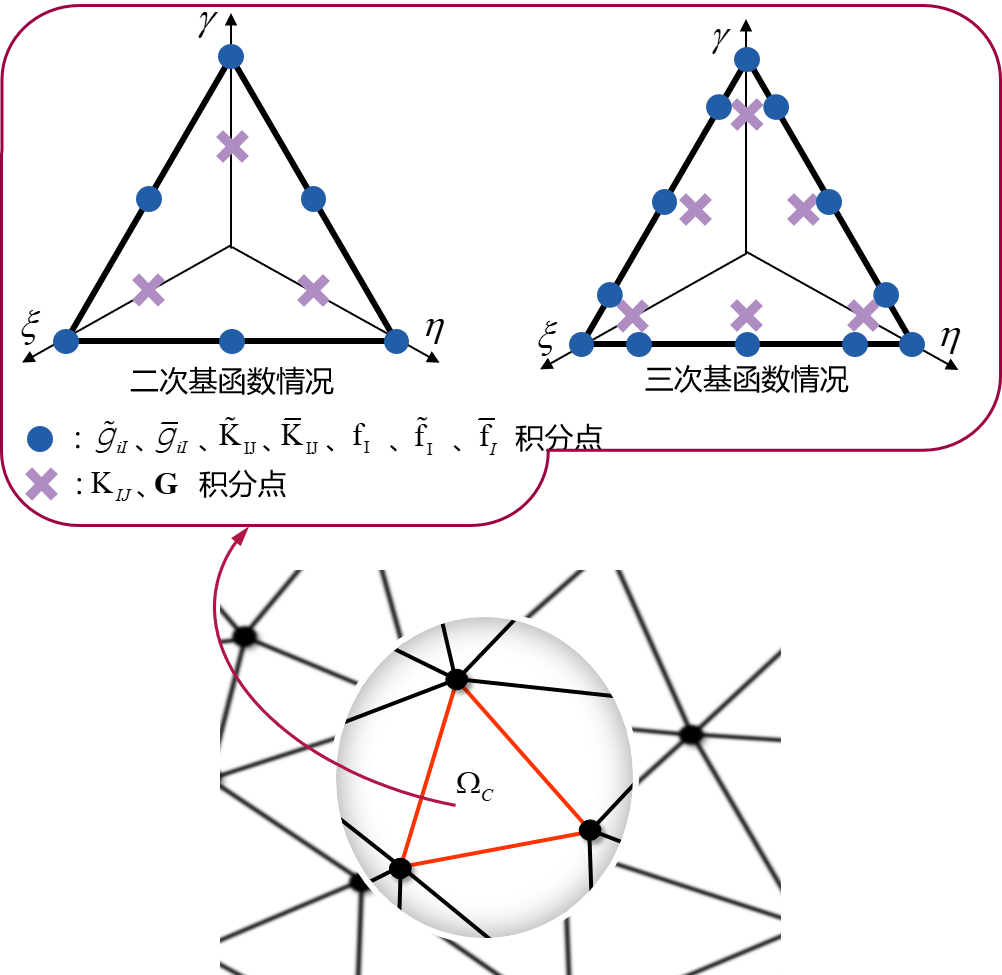
\includegraphics[scale=0.6]{figure/EHR/Eintegralscheme.png}
    \caption{优化的数值积分方案}\label{Eintegralscheme}
\end{figure}
基于Hellinger-Reissner变分原理的本质边界条件施加方法中,再生光滑梯度的构造过程需要计算积分点处的无网格形函数,此时为了减少形函数的计算量提高计算效率,采用无网格再生核光滑梯度积分法。
无网格再生核光滑梯度积分法利用积分点在背景积分单元间的共享特性,优化整体求解数值过程中积分点的数量,从而提高计算效率。
再生核光滑梯度积分法通过在背景积分单元上选择合适的积分点分布,使得积分点在不同单元之间共享,减少需要计算的积分点数量,进而保证计算精度的前提下进一步提高计算效率,
具体的数值积分方案见附录C无网格法优化的数值积分方案。
\section{数值算例}
\subsection{分片实验}
首先采用线性、二次和三次弹性力学分片实验验证采用传统高斯积分法和再生光滑梯度积分法的不同本质边界条件施加方法下是否满足积分约束条件的情况。
分片实验考虑求解域为边长等于1的正方形,求解域的四边施加本质边界条件。其分片实验的精确解如下:
\begin{equation}
\begin{split}
    \begin{cases}
        u_x(x,y)=(1+2x+3y)^n\\
        u_y(x,y)=(4+5x+6y)^n
    \end{cases}
\end{split}
\end{equation}
其中,$n=1,2,3$表示线性、二次和三次分片实验。如图(\ref{patchtestmeshfree})所示,分片实验采用$11\times 11$的非均匀节点离散求解域。针对二次基函数的无网格近似,采用线性和二次分片实验进行测试,核函数相对影响域在二次基函数情况下为2.5;
三次基函数的无网格近似采用二次和三次分片实验进行测试,核函数相对影响域在三次基函数情况下为3.5。\par
分别采用位移误差$L_2$-Error和能量误差$H_1$-Error详细对比所提方法的计算精度
\begin{equation}
\begin{split}
    L_2\text{-Error}=\sqrt{\int_{\Omega}(u_i-u_i^h)(u_i-u_i^h)d\Omega}
\end{split}
\end{equation}
\begin{equation}
    \begin{split}
        H_1\text{-Error}=\sqrt{\frac{1}{2}\int_{\Omega}(\sigma_{ij}-\sigma_{ij}^h)C_{ijkl}^{-1}(\sigma_{ij}-\sigma_{ij}^h)d\Omega}
    \end{split}
    \end{equation}\par
\begin{figure}[H]
    \centering
    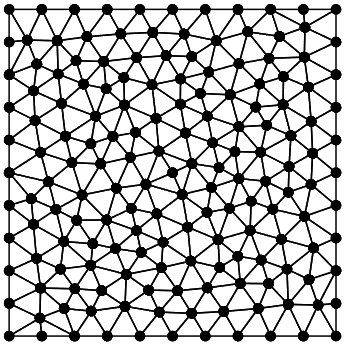
\includegraphics[scale=0.7]{figure/EHR/patchtestmeshfree.png}
    \caption{分片实验无网格离散模型}\label{patchtestmeshfree}
\end{figure} 
在数值结果中,“GI”表示采用的是传统高斯积分法,“RKGSI”表示采用的是再生光滑梯度积分法。“Penalty”、“LM”和“Nitsche”分别表示罚函数法、拉格朗日乘子法和Nitsche法三种常见的本质边界条件施加方法。“RKGSI-HR”则表示的是本章提出的
基于Hellinger-Reissner变分原理的本质边界条件施加方法。\par
在数值求解过程中,为了保证拉格朗日乘子法的稳定性,拉格朗日乘子统一采用线性有限元形函数进行离散。针对二次基函数的求解,高斯积分法“GI”的求解域$\Omega$的积分采用13点高斯积分,边界$\Gamma$积分采用3点高斯积分
;针对三次基函数的求解,高斯积分法“GI”的求解域$\Omega$的积分采用16点高斯积分,边界$\Gamma$积分采用5点高斯积分。二次和三次基函数的无网格法分片试验结果如下:\par
\begin{table}[H]
\caption{\textbf{二次基函数无网格法分片实验结果}}
\centering
\begin{tabular}{lcccc}
   \toprule
& \multicolumn{2}{c}{线性分片实验} & \multicolumn{2}{c}{二次分片实验} \\ \cline{2-5}
   &$L_2$-Error$\quad$&$H_1$-Error&$L_2$-Error$\quad$&$H_1$-Error\\
   \midrule
   GI-Penalty&$7.7\times10^{-6}$&$2.7\times10^{-4}$&$1.2\times10^{-5}$&$2.6\times10^{-4}$\\
   GI-LM&$1.0\times10^{-4}$&$4.7\times10^{-3}$&$1.5\times10^{-4}$&$4.3\times10^{-3}$\\
   GI-Nitsche&$8.1\times10^{-6}$&$2.8\times10^{-4}$&$1.3\times10^{-5}$&$2.8\times10^{-4}$\\
  RKGSI-Penalty&$7.9\times10^{-8}$&$2.0\times10^{-6}$&$1.4\times10^{-7}$&$2.1\times10^{-6}$\\
  RKGSI-LM&$8.6\times10^{-5}$&$4.0\times10^{-3}$&$1.4\times10^{-4}$&$3.7\times10^{-3}$\\
  RKGSI-Nitsche&$2.1\times10^{-15}$&$4.0\times10^{-14}$&$2.2\times10^{-15}$&$2.7\times10^{-14}$\\
  RKGSI-HR&$2.0\times10^{-15}$&$3.2\times10^{-14}$&$2.2\times10^{-15}$&$2.1\times10^{-14}$\\
\bottomrule
\end{tabular}
\end{table}
\begin{table}[H]
\caption{\textbf{三次基函数无网格法分片实验结果}}
\centering
\begin{tabular}{lcccc}
   \toprule
& \multicolumn{2}{c}{二次分片实验} & \multicolumn{2}{c}{三次分片实验} \\ \cline{2-5}
   &$L_2$-Error$\quad$&$H_1$-Error&$L_2$-Error$\quad$&$H_1$-Error\\
   \midrule
   GI-Penalty&$9.1\times10^{-6}$&$2.1\times10^{-4}$&$1.2\times10^{-5}$&$2.0\times10^{-4}$\\
   GI-LM&$2.9\times10^{-4}$&$9.3\times10^{-3}$&$4.0\times10^{-4}$&$9.3\times10^{-3}$\\
   GI-Nitsche&$1.1\times10^{-5}$&$2.8\times10^{-4}$&$1.4\times10^{-5}$&$2.7\times10^{-4}$\\
  RKGSI-Penalty&$1.4\times10^{-7}$&$2.1\times10^{-6}$&$2.0\times10^{-7}$&$2.7\times10^{-6}$\\
  RKGSI-LM&$3.0\times10^{-4}$&$9.8\times10^{-3}$&$4.2\times10^{-4}$&$9.8\times10^{-3}$\\
  RKGSI-Nitsche&$3.6\times10^{-15}$&$1.0\times10^{-13}$&$4.6\times10^{-15}$&$9.5\times10^{-14}$\\
  RKGSI-HR&$3.1\times10^{-15}$&$1.0\times10^{-13}$&$3.5\times10^{-15}$&$7.4\times10^{-14}$\\
   \bottomrule
\end{tabular}
\end{table}
表3.3和表3.4分别为具有二次、三次基函数无网格法的分片试验结果,
从表中可以看出,由于传统高斯积分法不满足积分约束条件,所以即使采用高阶高斯积分的罚函数法“GI-Penalty”、拉格朗日乘子法“GI-LM”和Nitsche法“GI-Nitsche”均不能通过分片试验。
当采用满足积分约束条件的再生光滑梯度积分法时,此时由于罚函数法“RKGSI-Penalty”不具有变分一致性,也无法通过分片试验;
拉格朗日乘子法“RKGSI-LM”由于其拉格朗日乘子采用线性形函数进行离散,无法与再生光滑梯度相匹配,也无法通过分片试验;
当采用Nitsche法“RKGSI-Nitsche”和基于Hellinger-Reissner变分原理“RKGSI-HR”的本质边界条件施加方法时,均可以通过分片试验,即满足积分约束条件。
\subsection{悬臂梁问题}
首先考虑经典弹性力学二维悬臂梁问题,如图(\ref{cantilever})所示,悬臂梁的长和宽分别为$L=48$,$D=12$,同时悬臂梁的左端为固定支座,
右端沿着$y$轴正方向施加外部荷载$P=1000$。悬臂梁的材料系数为杨氏模量$E=3\times10^6$、泊松比$\nu=0.3$。
根据圣维南原理和平面应力假设,悬臂梁问题的解析解为:
\begin{equation}
\begin{split}
\begin{cases}
    u = -\frac{Py}{6EI}[(6L-3x)x + (2+\nu)(y^2 - \frac{D^2}{4})] \\
    v = \frac{P}{6EI}[3\nu y^2(L-x) + (4+5\nu)\frac{D^2x}{4} + (3L-x)x^2]
\end{cases}
\end{split}
\end{equation}
与之相对应的应力分量为:
\begin{equation}
\begin{split}
\begin{cases}
   \sigma_{xx}=-\frac{P(L-x)y}{I}\\
   \sigma_{yy}=0\\
   \sigma_{xy}=\frac{P}{2I}(\frac{D^2}{4}-y^2)
\end{cases}
\end{split}
\end{equation}
\begin{figure}[H]
    \centering
    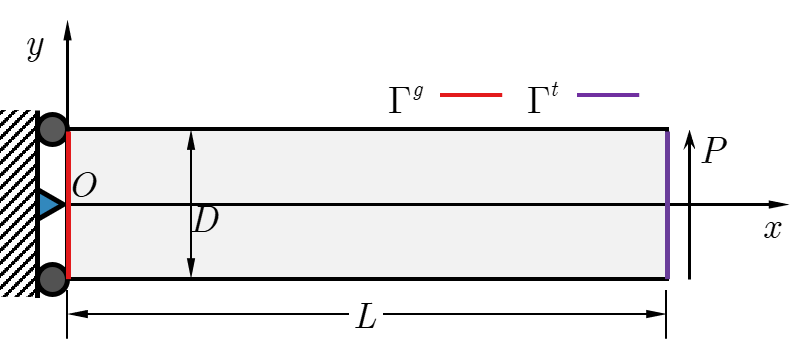
\includegraphics[scale=0.7]{figure/EHR/cantilever/cantilever.png}
    \caption{悬臂梁问题模型}\label{cantilever}
\end{figure}
如图(\ref{cantilever})所示,悬臂梁的左端施加自然边界条件$\Gamma^t$,右端施加本质边界条件$\Gamma^g$。
悬臂梁求解域分别通过图(\ref{cantilever.mesh})所示采用四个疏密不同的节点进行离散。对于采用二次基函数的悬臂梁算例问题,传统高斯积分法采用13点高斯积分,核函数的相对影响域为2.5。
\newpage
\begin{figure}[H]
    \centering
    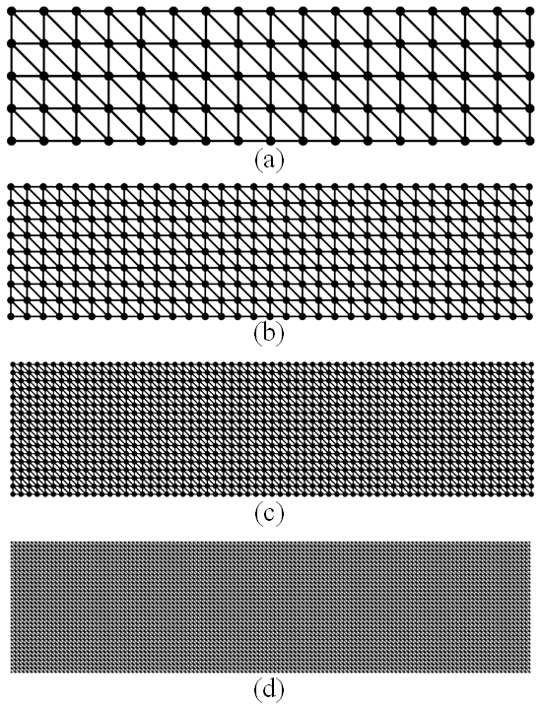
\includegraphics[scale=0.8]{figure/EHR/cantilever/cantilever.mesh.png}
    \caption{悬臂梁问题节点模型}\label{cantilever.mesh}
\end{figure}
图(\ref{ECLH})为悬臂梁问题的位移误差和能量误差对比图。从图中可以看出采用再生光滑梯度积分法“RKGSI”的本质边界条件施加方法的计算精度优于采用高斯积分法“GI”的本质条件施加方法,
并且由于传统高斯积分法和采用再生光滑梯度积分法的罚函数法“RKGSI-Penalty”和拉格朗日乘子法“RKGSI-LM”不具有变分一致性,无法达到理论误差收敛率,而基于Hellinger-Reissner变分原理下的本质边界条件施加方法“RKGSI-HR”和Nitshce法“RKGSI-Nitsche”均可达到理论误差收敛率,但相较于“RKGSI-Nitsche”法,所提出的“RKGSI-HR”法无需引入人工参数。
\par
图(\ref{ECcputime})为悬臂梁问题的节点数和计算时间的效率对比和本质边界条件施加效率对比图。从整体来看采用再生光滑梯度积分法“RKGSI”的计算效率明显高于传统高斯积分法“GI”。
图(\ref{ECefficiency})为悬臂梁问题的本质边界条件施加效率分析图。该图为施加本质边界$\Gamma^g$过程中计算形函数及梯度和组装相对应的刚度矩阵和力向量所用时间对比图。
从图中可以看出,罚函数法和拉格朗日乘子法在计算形函数及其梯度所用的时间相同且所用时间最少,这是由于罚函数法和拉格朗日乘子法在计算过程中只需要计算无网格形函数本身,无需计算无网格形函数梯度,
而“RKGSI-HR”法也无需计算无网格形函数梯度,但需要计算再生光滑梯度,“RKGSI-Nitsche”法这部分所用的时间是罚函数法和拉格朗日乘子法的5.6倍,而“RKGSI-HR”法是1.6倍,“RKGSI-HR”法的计算效率高于“RKGSI-Nitsche”法。
组装相应的刚度矩阵和力向量这部分所用的时间上,“RKGSI-Nitsche”法和“RKGSI-HR”法计算效率基本相同。
从整体上来看,拉格朗日乘子法和罚函数法的效率优于“HR”法和“Nitsche”法,但拉格朗日乘子法和罚函数法不具有变分一致性无法达到理论误差收敛率。
因此,总体来说,相较于传统的本质边界条件施加方法,基于Hellinger-Reissner变分原理的本质边界条件施加方法“RKGSI-HR”能够达到理论误差收敛率,有效提高计算精度,相较于“RKGSI-Nitsche”法而言计算效率也更高。
\begin{figure}[H]
\centering
\begin{subcaptiongroup}
    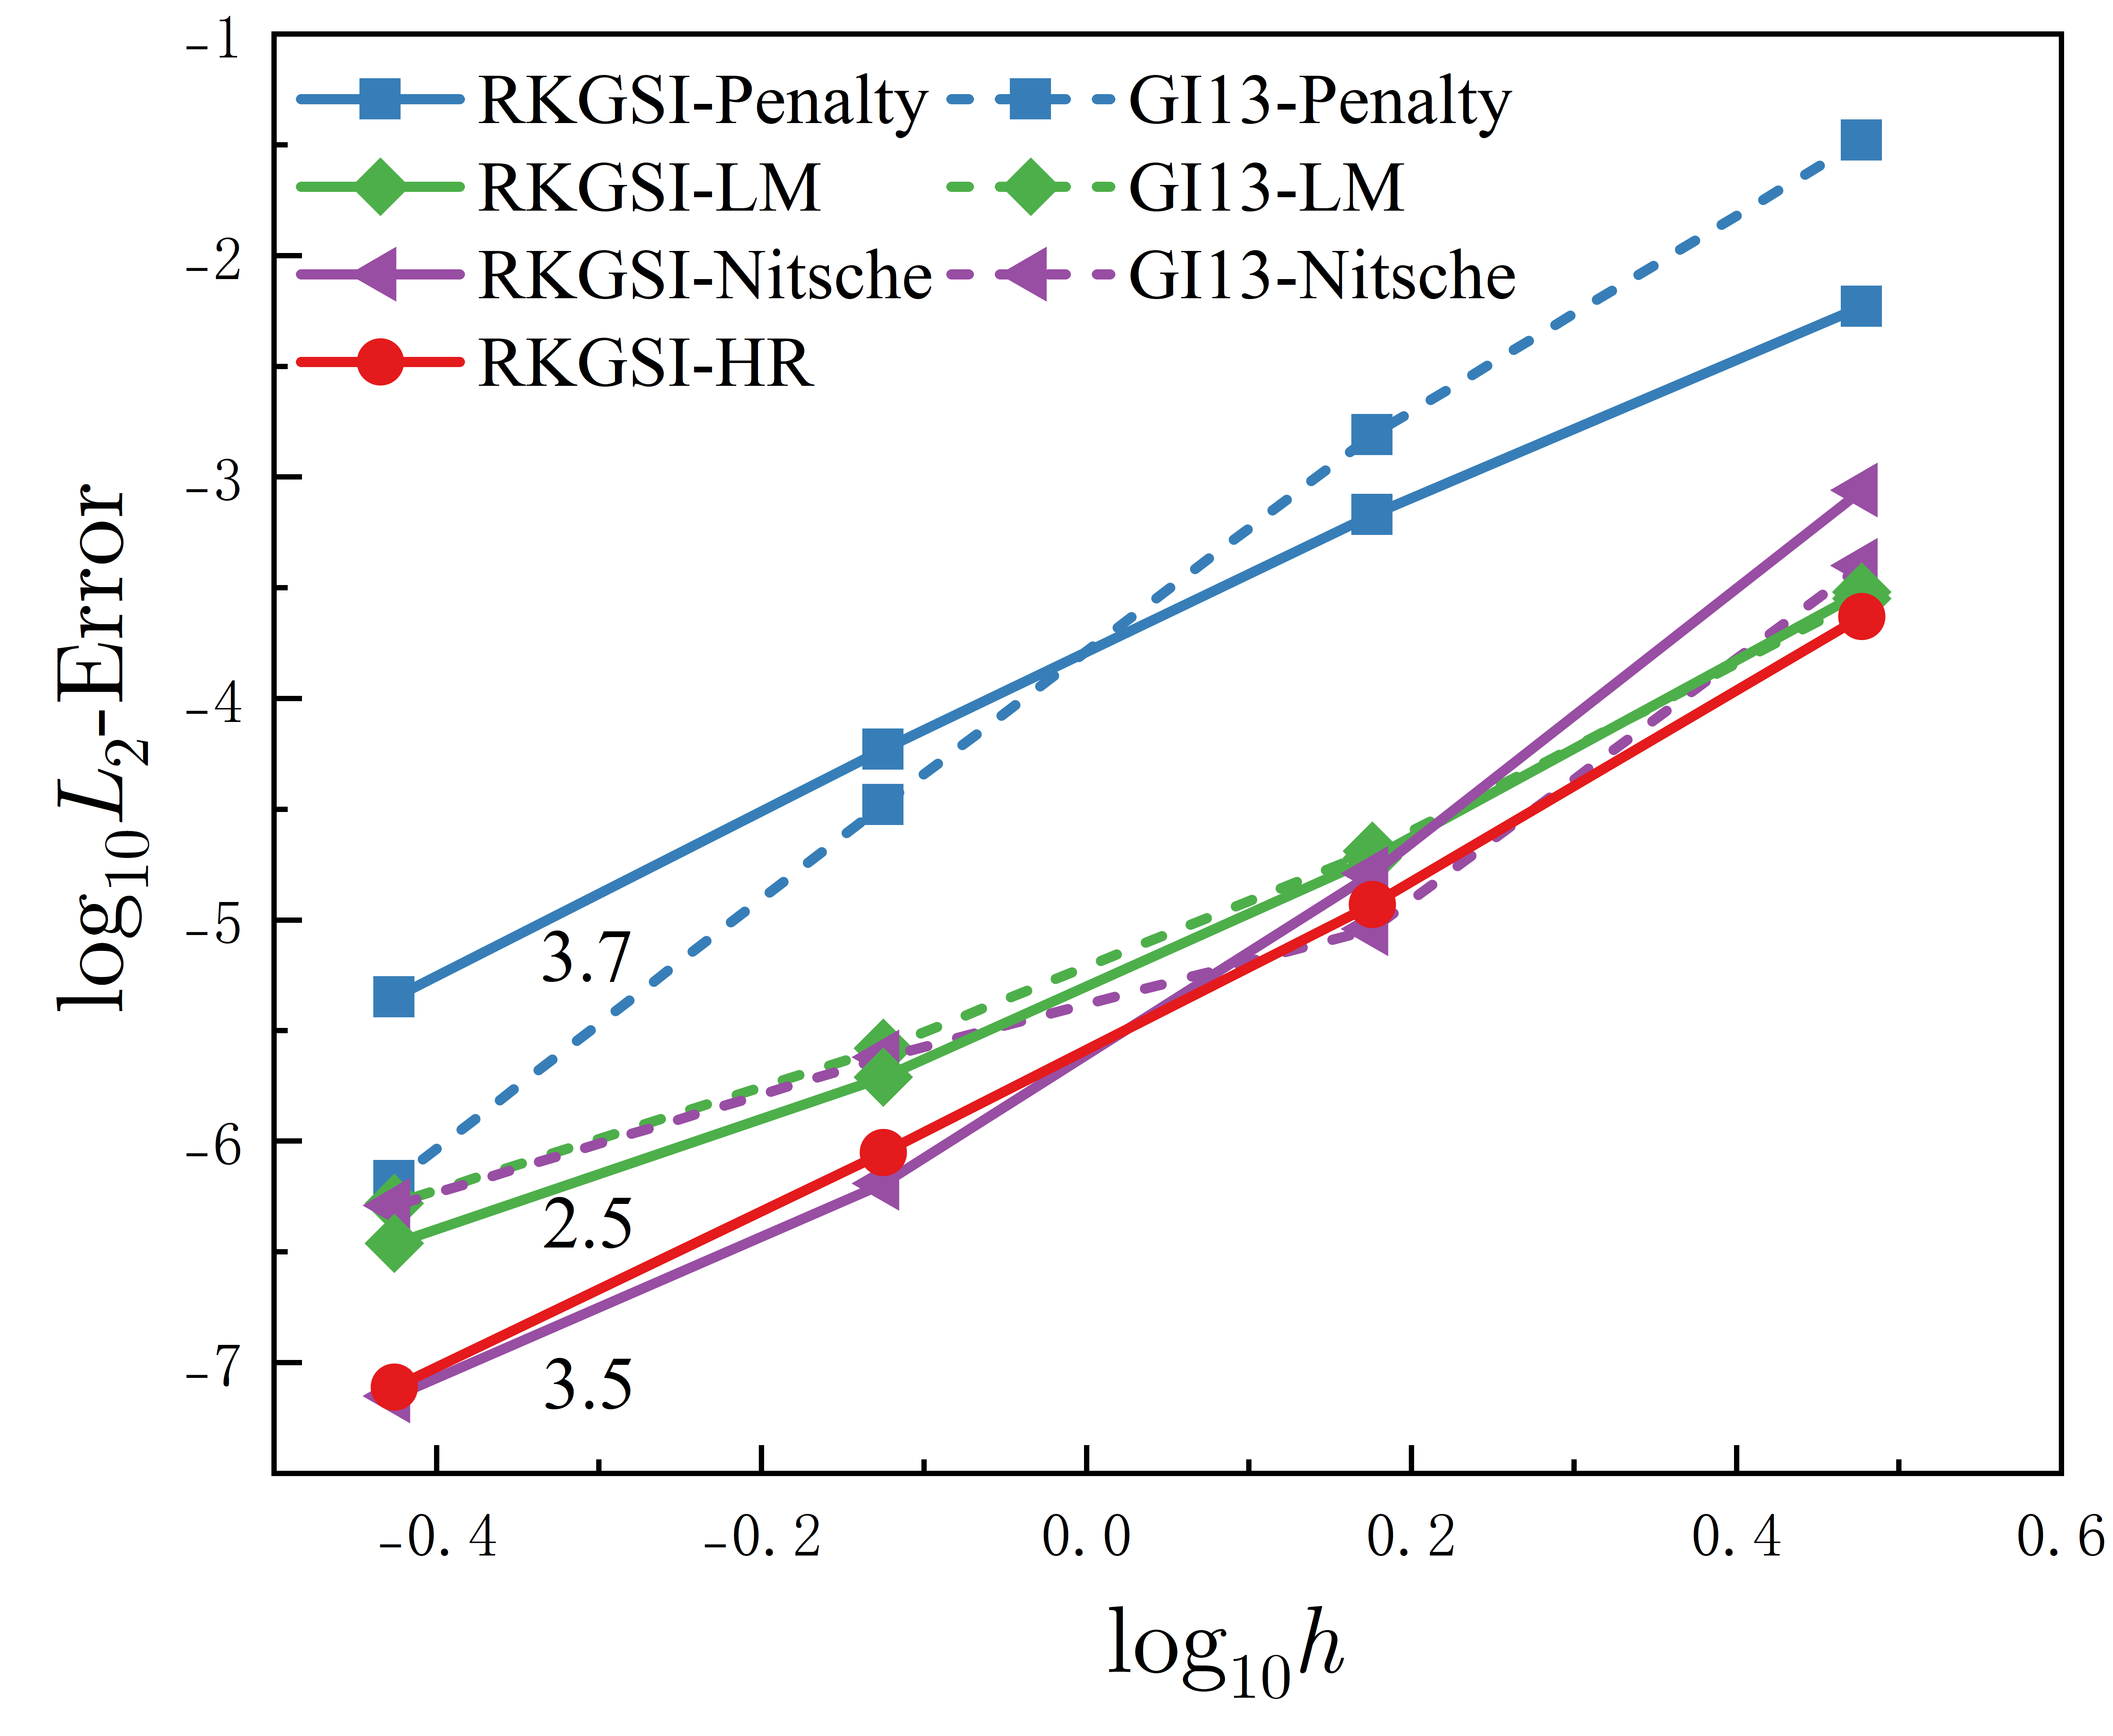
\includegraphics[width=0.49\textwidth]{figure/EHR/cantilever/L2.png}
    \phantomcaption\label{ECL2}
    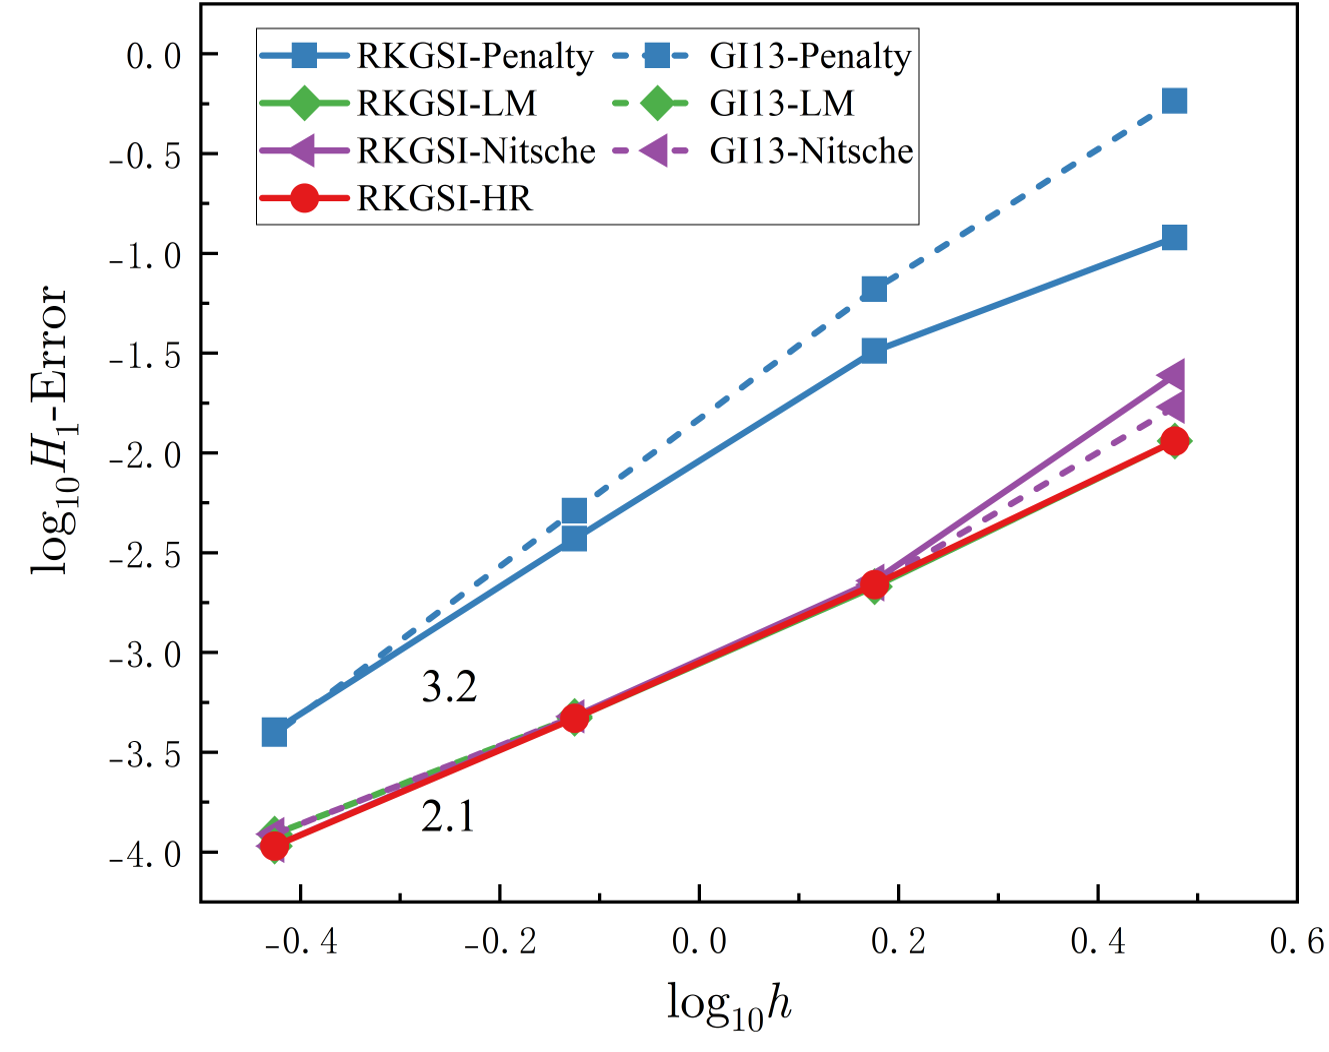
\includegraphics[width=0.49\textwidth]{figure/EHR/cantilever/H1.png}
    \phantomcaption\label{ECH1}
    \end{subcaptiongroup}
\caption{悬臂梁问题误差对比:\subref{ECL2} $L_2$误差;\subref{ECH1} $H_1$误差}
\label{ECLH}
\end{figure}
\begin{figure}[H]
\centering
    \begin{subcaptiongroup}
        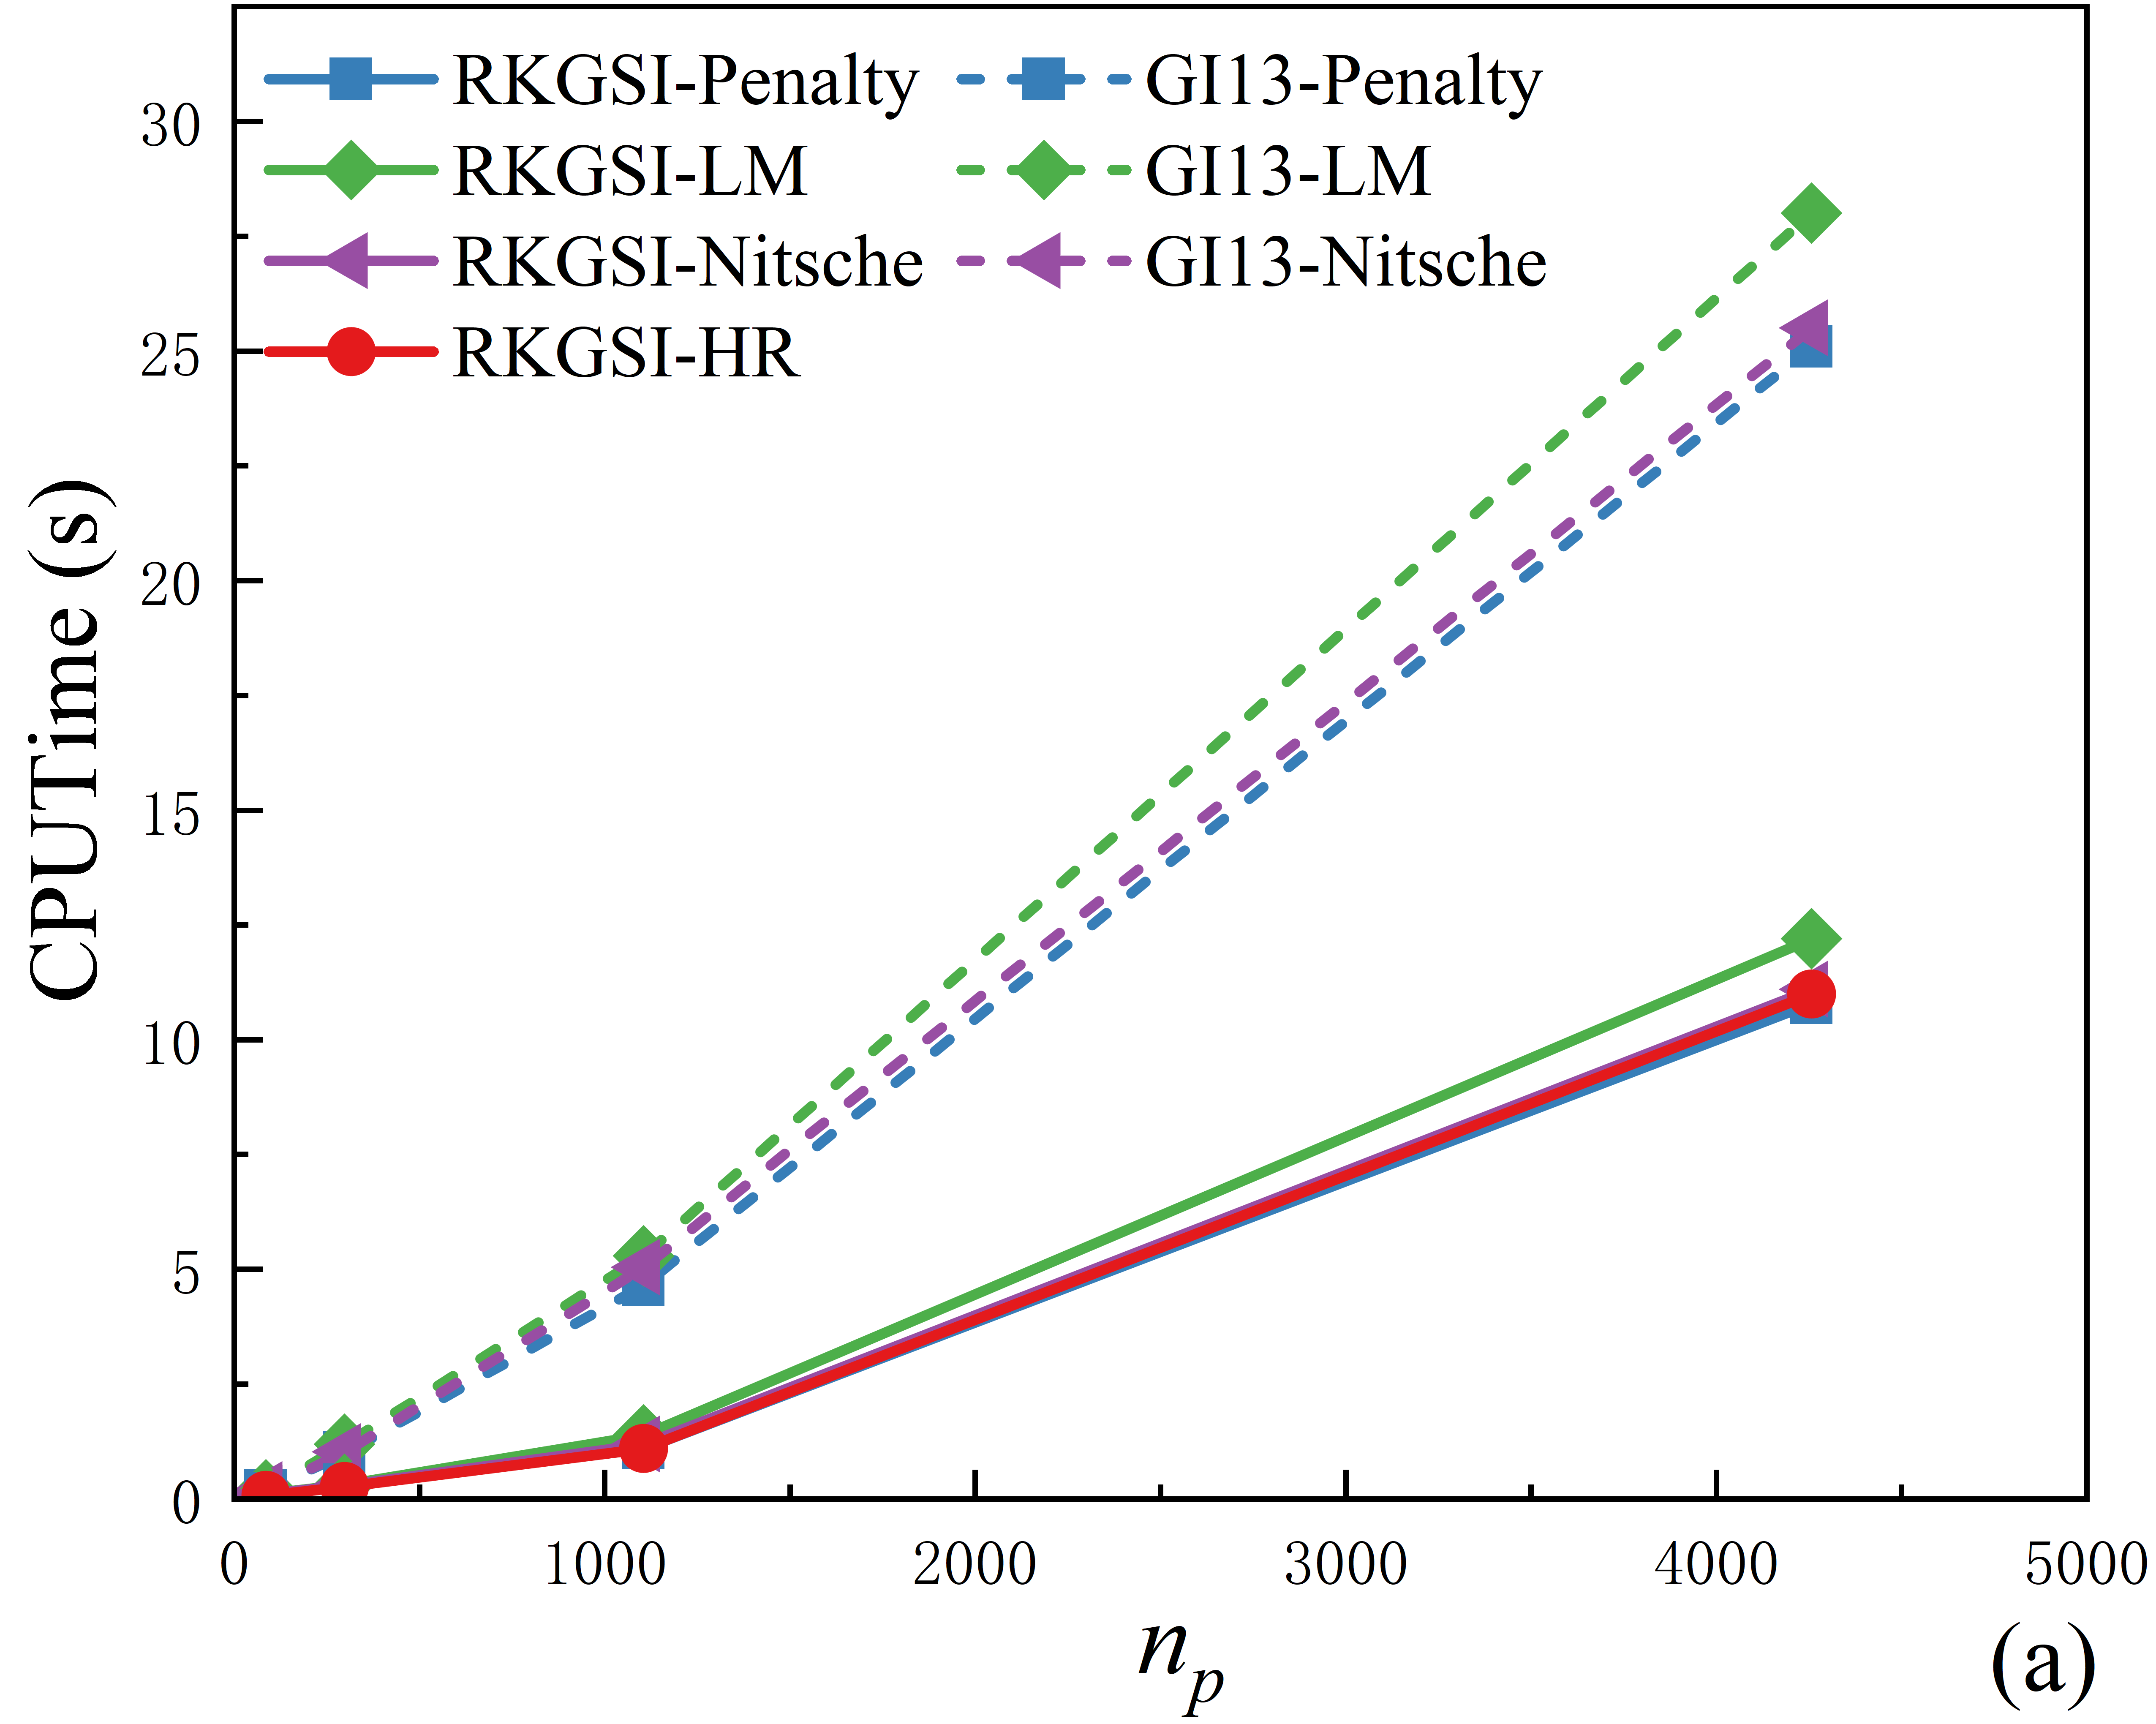
\includegraphics[width=0.49\textwidth]{figure/EHR/cantilever/cputime.png}
        \phantomcaption\label{ECcputime}
        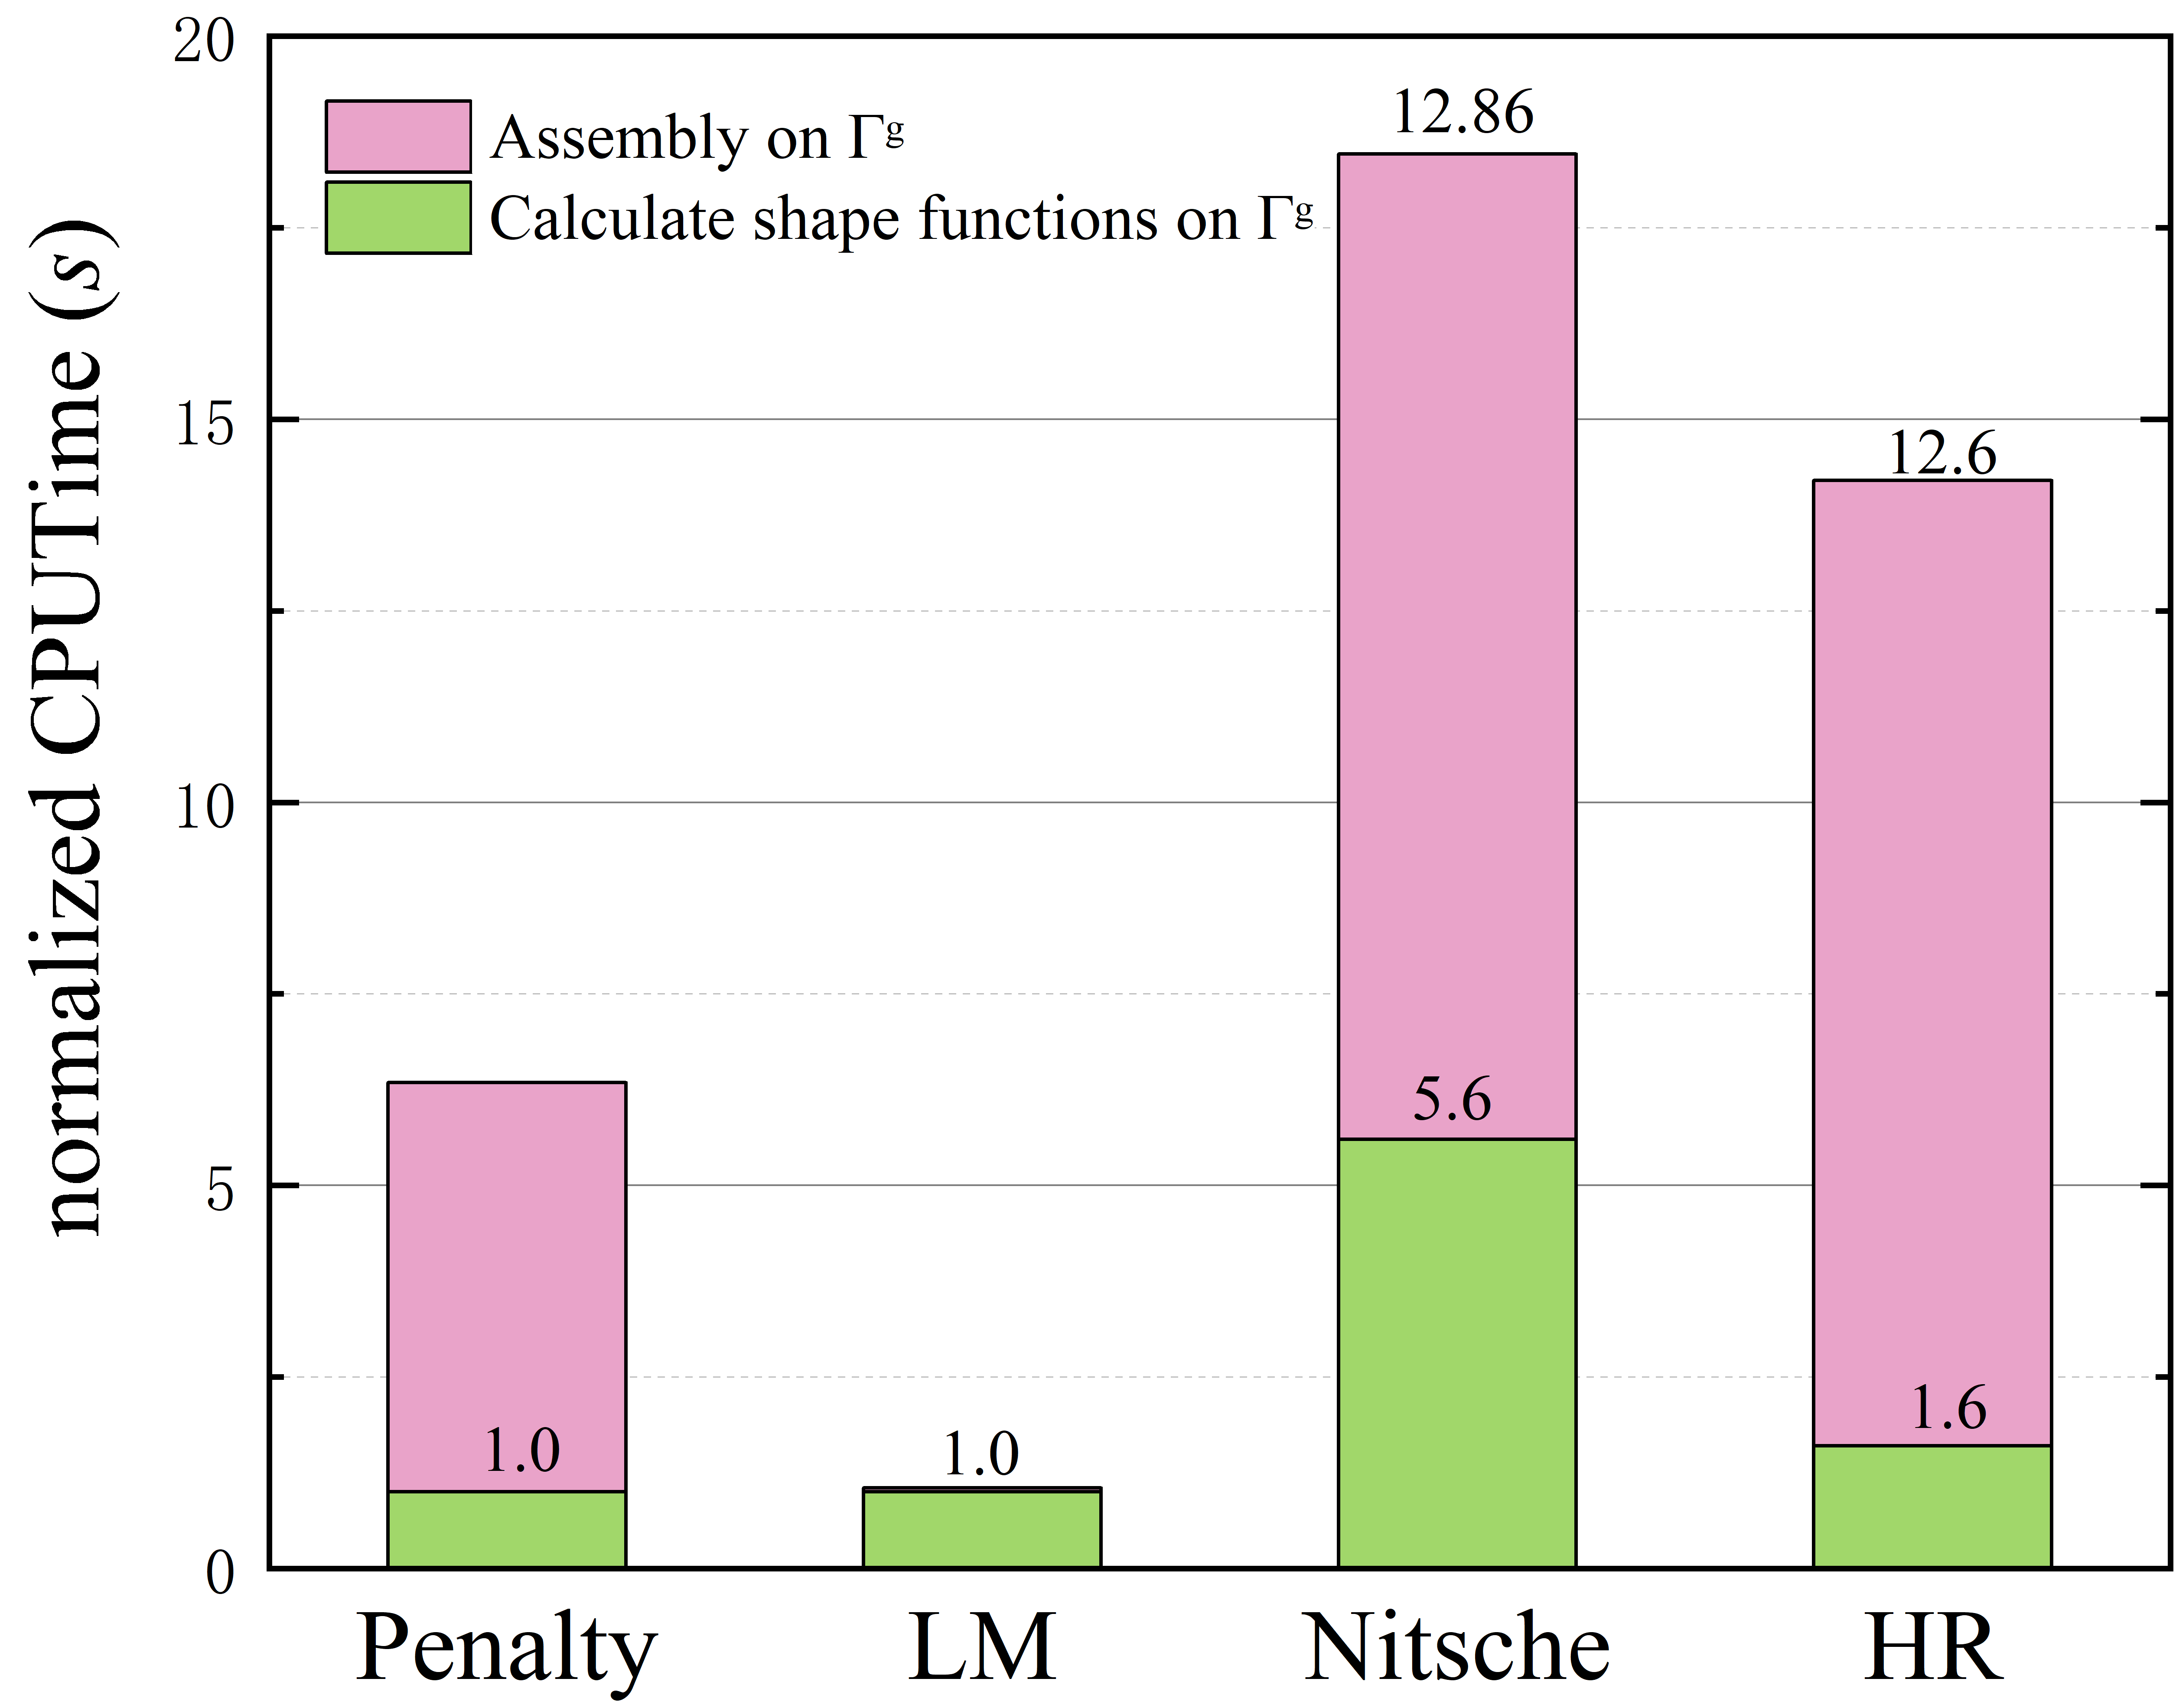
\includegraphics[width=0.49\textwidth]{figure/EHR/cantilever/efficiency.png}
        \phantomcaption\label{ECefficiency}
        \end{subcaptiongroup}
\caption{悬臂梁问题效率对比:\subref{ECcputime} 计算时间与节点数的关系;\subref{ECefficiency} 边界条件施加效率分析}
\end{figure}
\subsection{带孔无限大平板问题}
考虑经典的带孔无限大平板问题,如图(\ref{hole})所示,板的的中心存在一半径为$a=1$的圆形小孔,同时平板的无穷远处沿$x$轴方向施加均布荷载$T=1000$。
板的材料系数为杨氏模量$E=3\times10^6$、泊松比$\nu=0.3$。根据Michell解可以得到该带孔无限大平板问题的解析解为:
\begin{equation}
\begin{split}
\begin{cases}
    u_x(r,\theta)=\frac{Ta}{8\mu}(\frac{r}{a}(k+1)cos\theta-\frac{2a^3}{r^3}cos3\theta+\frac{2a}{r}((1+k)cos\theta+cos3\theta))\\
    u_y(r,\theta)=\frac{Ta}{8\mu}(\frac{r}{a}(k-3)sin\theta-\frac{2a^3}{r^3}sin3\theta+\frac{2a}{r}((1-k)sin\theta+sin3\theta))  
\end{cases}
\end{split}
\end{equation}
其中,$k$和$\mu$分别为:
\begin{equation}
\begin{split}
    k=\frac{3-\nu}{1+\nu}\quad \text{,}\mu=\frac{E}{2(1+\nu)}
\end{split}
\end{equation}
与之相对应的应力分量为:
\begin{equation}
\begin{split}
\begin{cases}
    \sigma_{xx}=T(1-\frac{a^2}{r^2}(\frac{3}{2}cos2\theta+cos4\theta)+\frac{3a^4}{2r^4}cos4\theta)\\
    \sigma_{yy}=-T(\frac{a^2}{r^2}(\frac{1}{2}cos2\theta-cos4\theta)+\frac{3a^4}{2r^4}cos4\theta)\\
    \sigma_{xy}=-T(\frac{a^2}{r^2}(\frac{1}{2}sin2\theta+sin4\theta)-\frac{3a^4}{2r^4}sin4\theta)\\
\end{cases}
\end{split}
\end{equation}\par
如图(\ref{hole})所示,根据带孔无限大平板的对称性,取边长$b=5$的四分之一的方形域作为研究对象。
方形域的上端和右端以及圆孔的边界施加自然边界条件$\Gamma^t$,而方形域的左端和下端约束法向位移,施加本质边界条件$\Gamma^g$。
\begin{figure}[H]
\centering
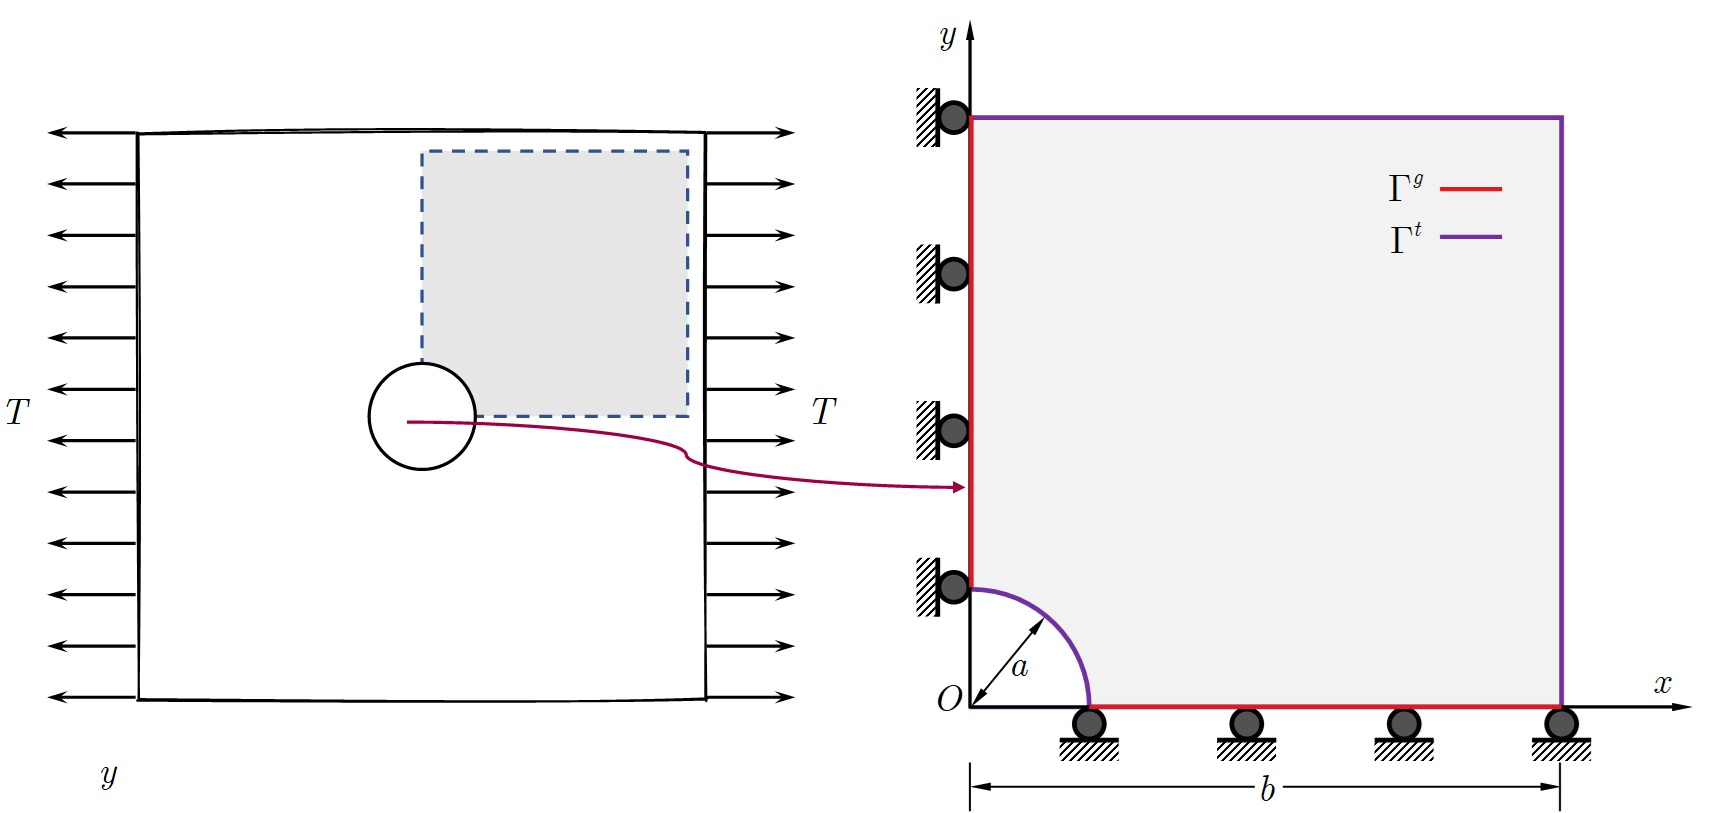
\includegraphics[scale=0.5]{figure/EHR/hole/hole.png}
    \caption{带孔无限大平板问题模型}\label{hole}
\end{figure}
该求解域分别通过图(\ref{hole.mesh})所示采用的四个疏密不同的节点进行离散。
对于采用三次基函数的带孔无限大平板算例问题,传统高斯积分法采用16点高斯积分,核函数的相对影响域为3.5。\par
\begin{figure}[H]
\centering
 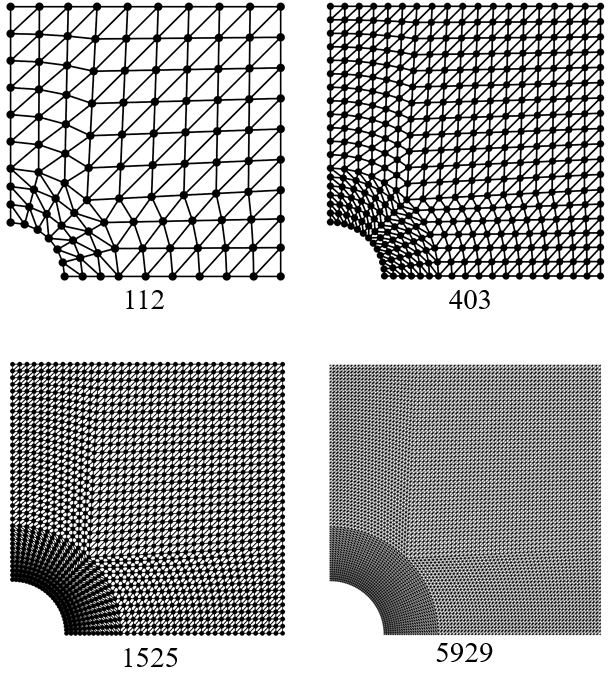
\includegraphics[scale=0.8]{figure/EHR/hole/hole.mesh.png}
   \caption{带孔无限大平板问题无网格离散}\label{hole.mesh}
\end{figure}
图(\ref{EHLH})为带孔无限大平板问题的位移和能量误差对比图。
从图中可以看出传统高斯积分法由于不具有变分一致性,导致“GI-Penalty”法、“GI-LM”法、“GI-Nitsche”法均无法达到理论误差收敛率。
基于Hellinger-Reissner变分原理的本质边界条件施加方法“RKGSI-HR”和“RKGSI-Nitsche”法满足变分一致性能够达到理论误差收敛率。
虽然“RKGSI-LM”法无法通过分片实验不满足变分一致性,但由于拉格朗日乘子法具有较高的精度也能达到理论误差收敛率。
图(\ref{Hcputime})、(\ref{Hefficiency})为带孔无限大平板问题的效率对比图。
从图中可以看出随着无网格节点数的增加,采用再生光滑梯度积分法“RKGSI”的效率明显高于传统高斯积分法“GI”,在施加本质边界条件的过程中,“HR”法不仅满足变分一致性同时计算效率还高于传统的“Nitsche”法。
最后,图(\ref{sigmaxx})为带孔无限大平板问题的应力云图,从图中可以看出“RKGSI-Penalty”法和精确解之间是有差异的,
而“RKGSI-Nitsche”法和“RKGSI-HR”法是和精确解几乎相同。但“Nitsche”法是需要依靠人工经验参数并且计算效率也低于“HR”法。
\newpage
\begin{figure}[H]
\centering
\begin{subcaptiongroup}
        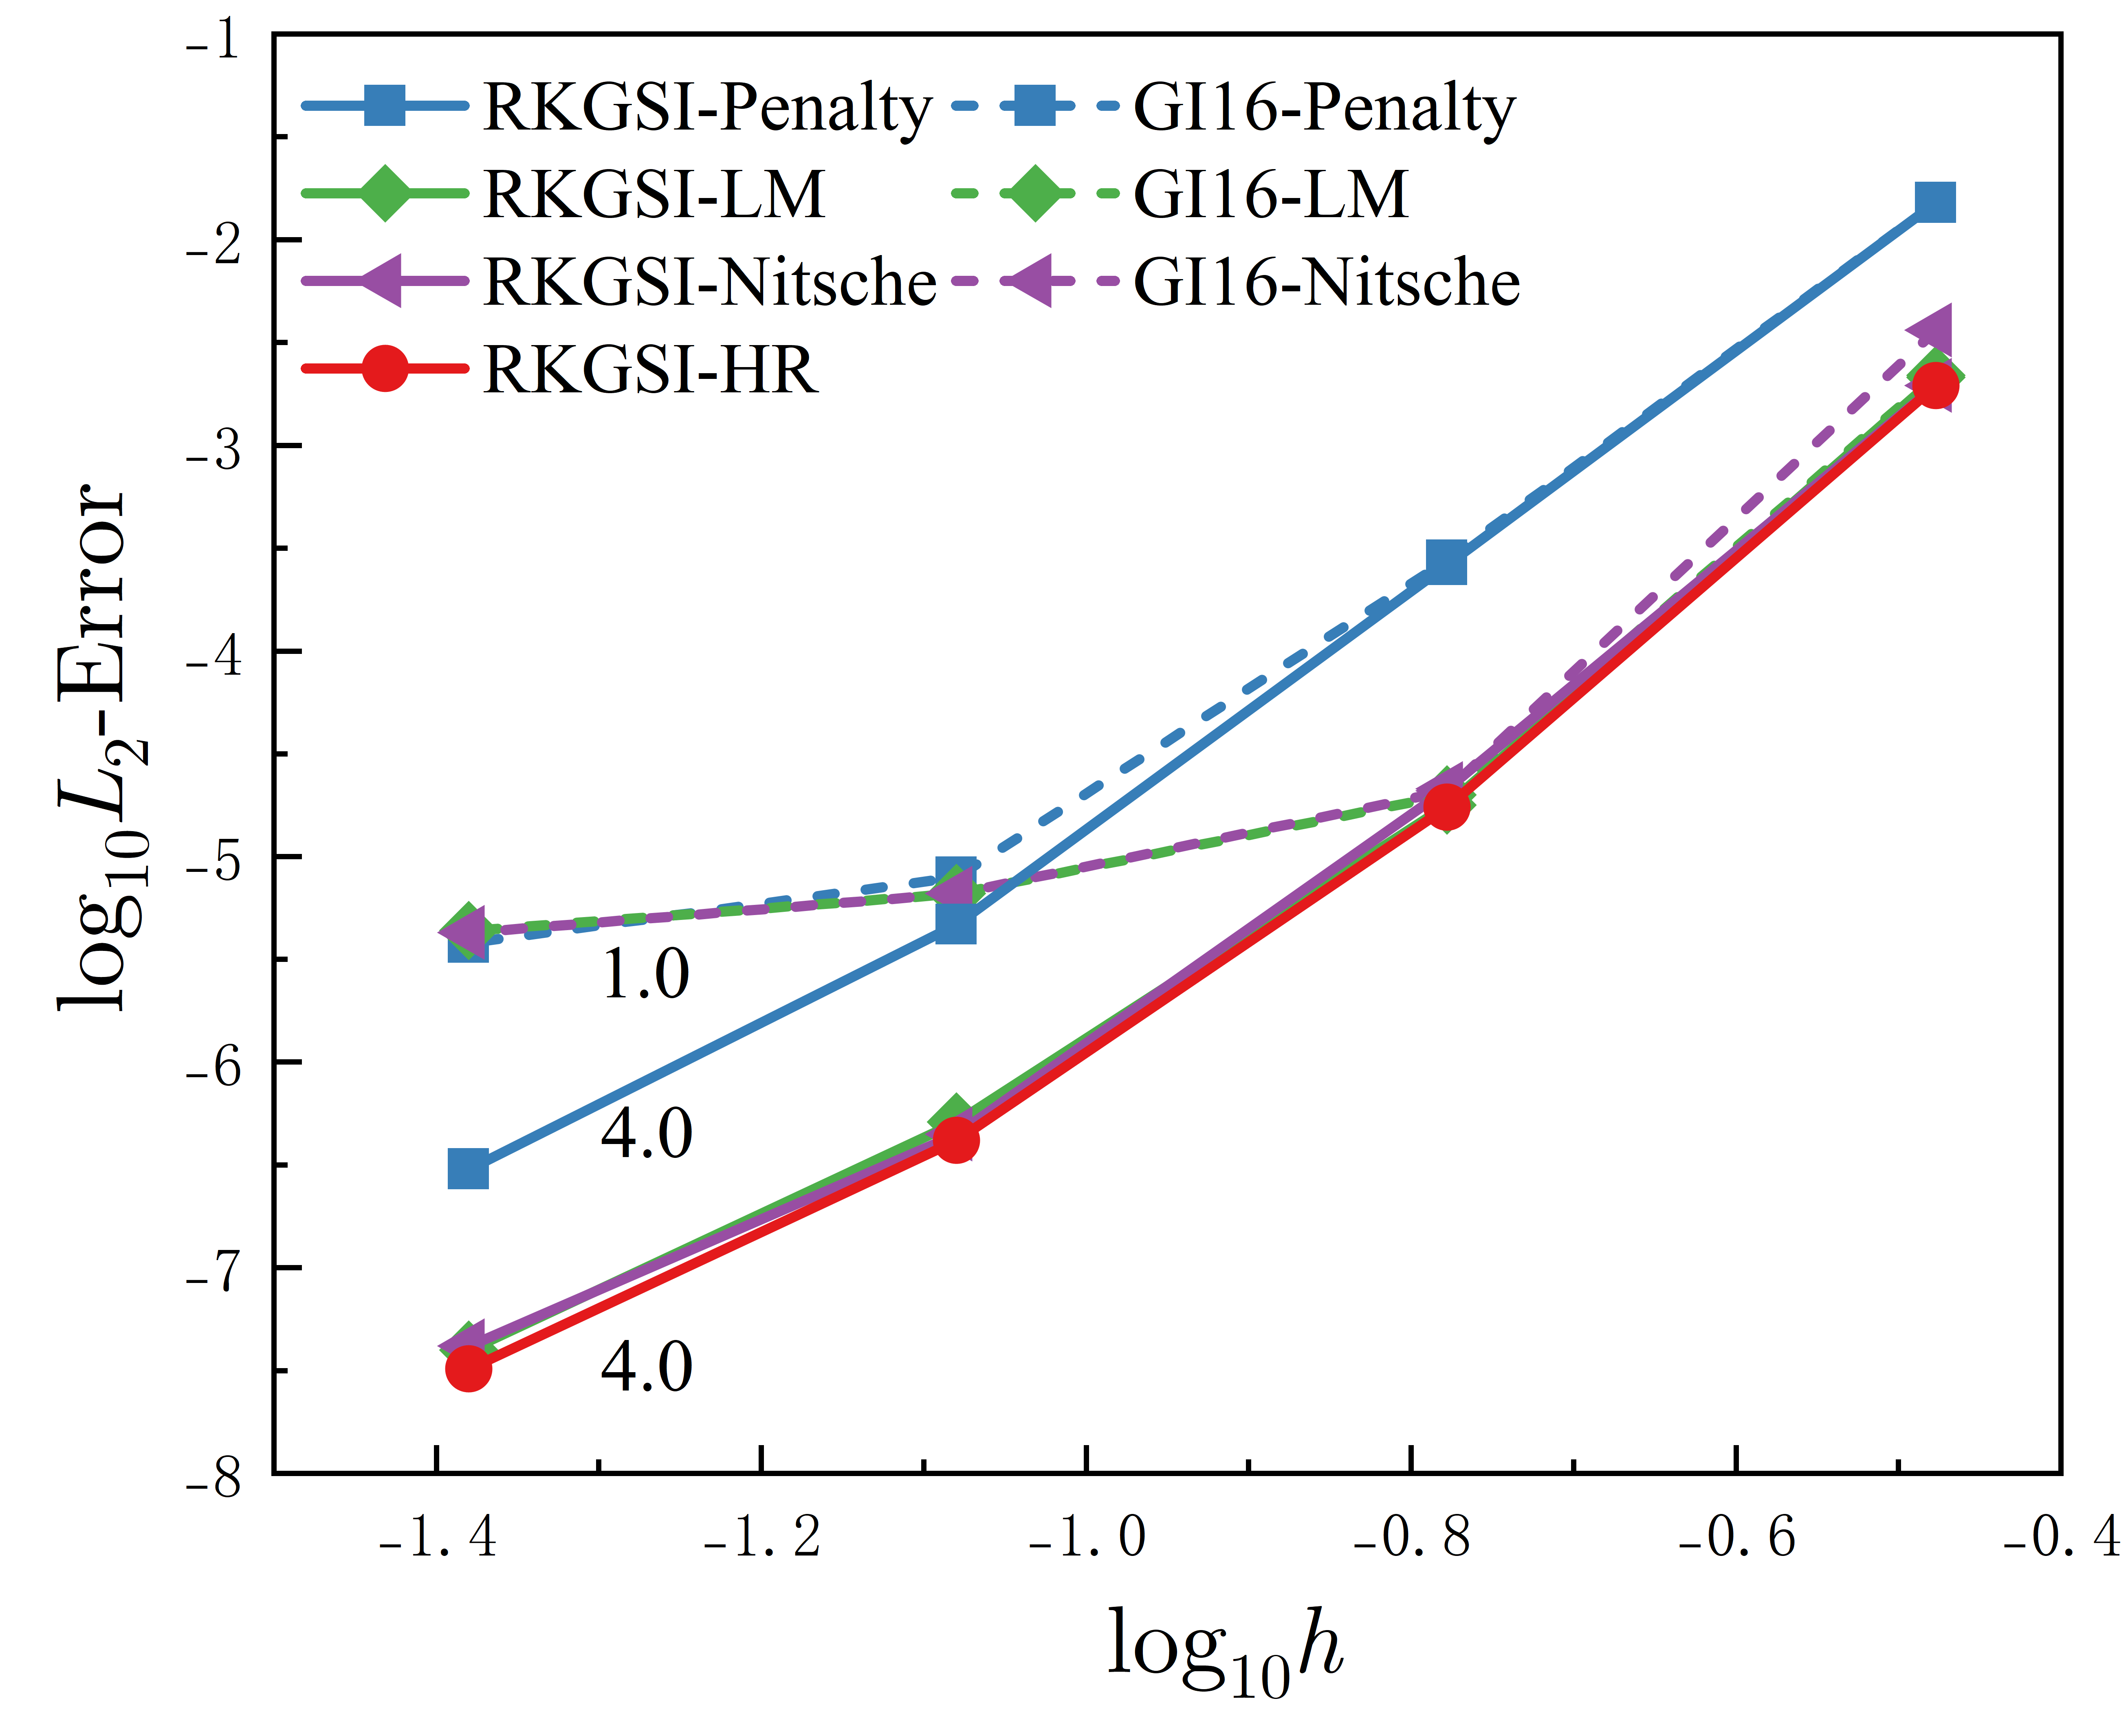
\includegraphics[width=0.49\textwidth]{figure/EHR/hole/L2.png}
        \phantomcaption\label{EHL2}
        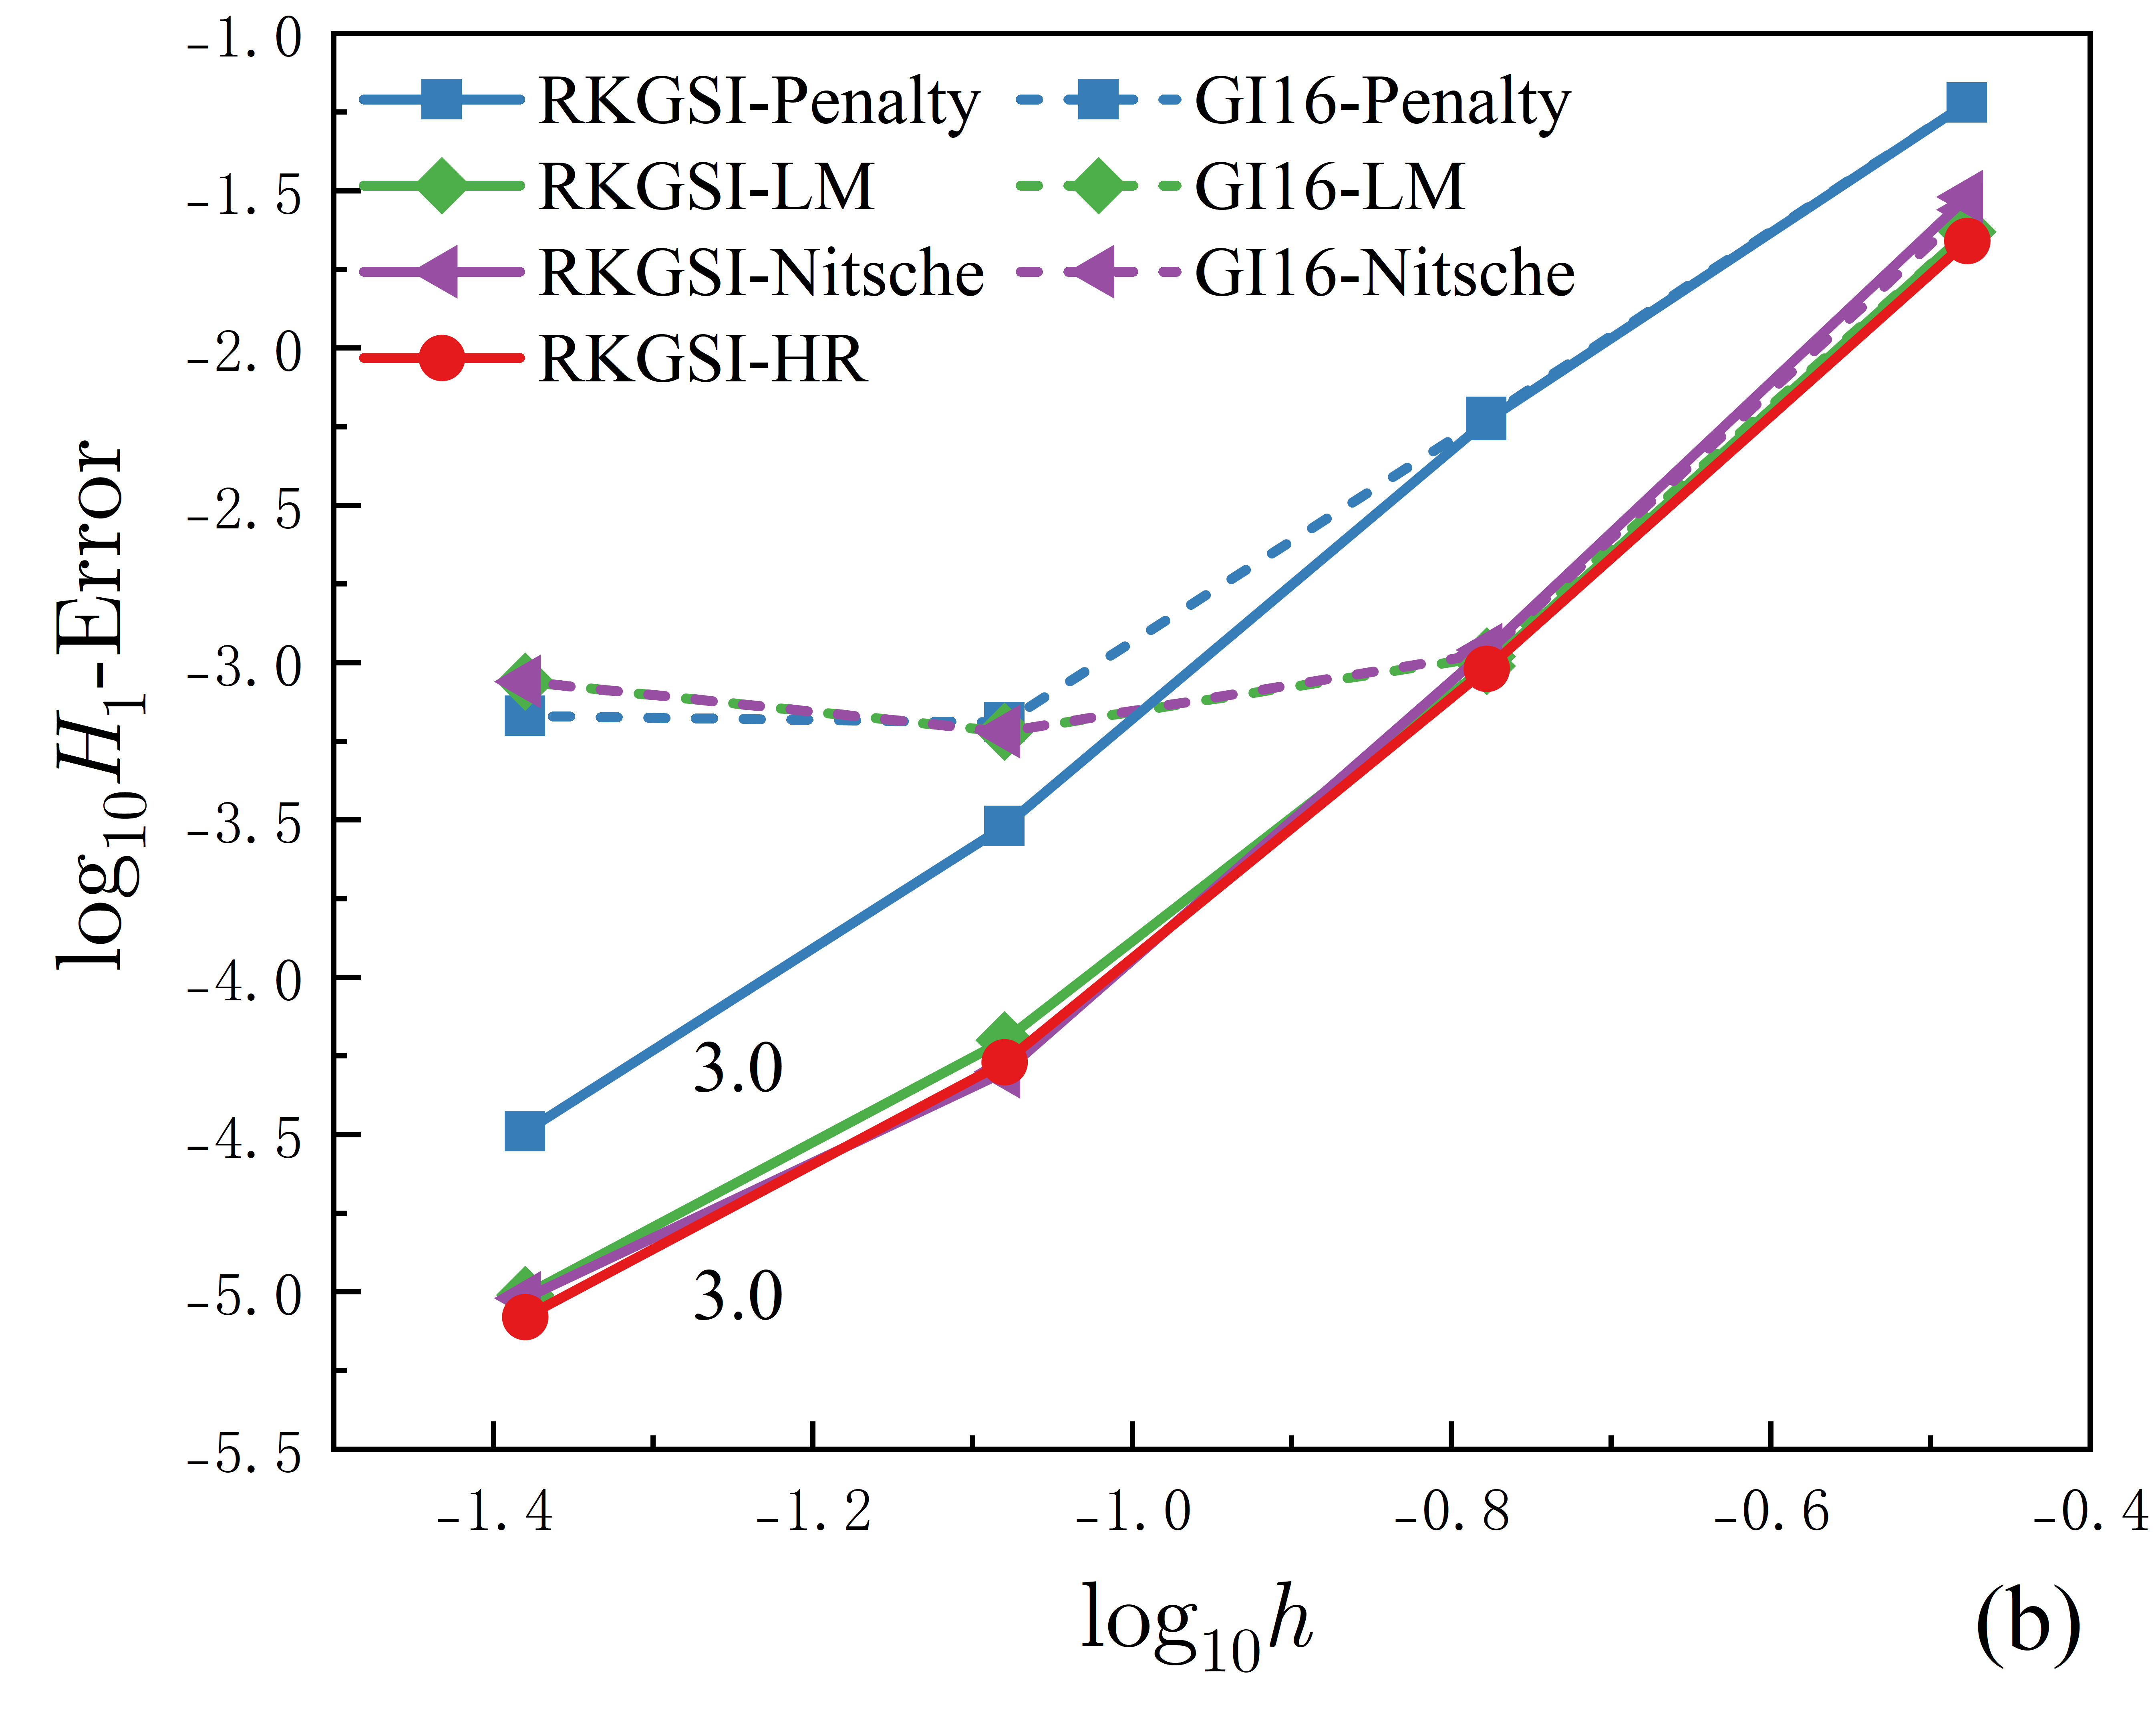
\includegraphics[width=0.49\textwidth]{figure/EHR/hole/H1.png}
        \phantomcaption\label{EHH1}
        \end{subcaptiongroup}
    \caption{带孔无限大平板问题误差对比:\subref{EHL2} $L_2$误差;\subref{EHH1} $H_1$误差}
    \label{EHLH}
    \end{figure}
\begin{figure}[H]
\centering
    \begin{subcaptiongroup}
    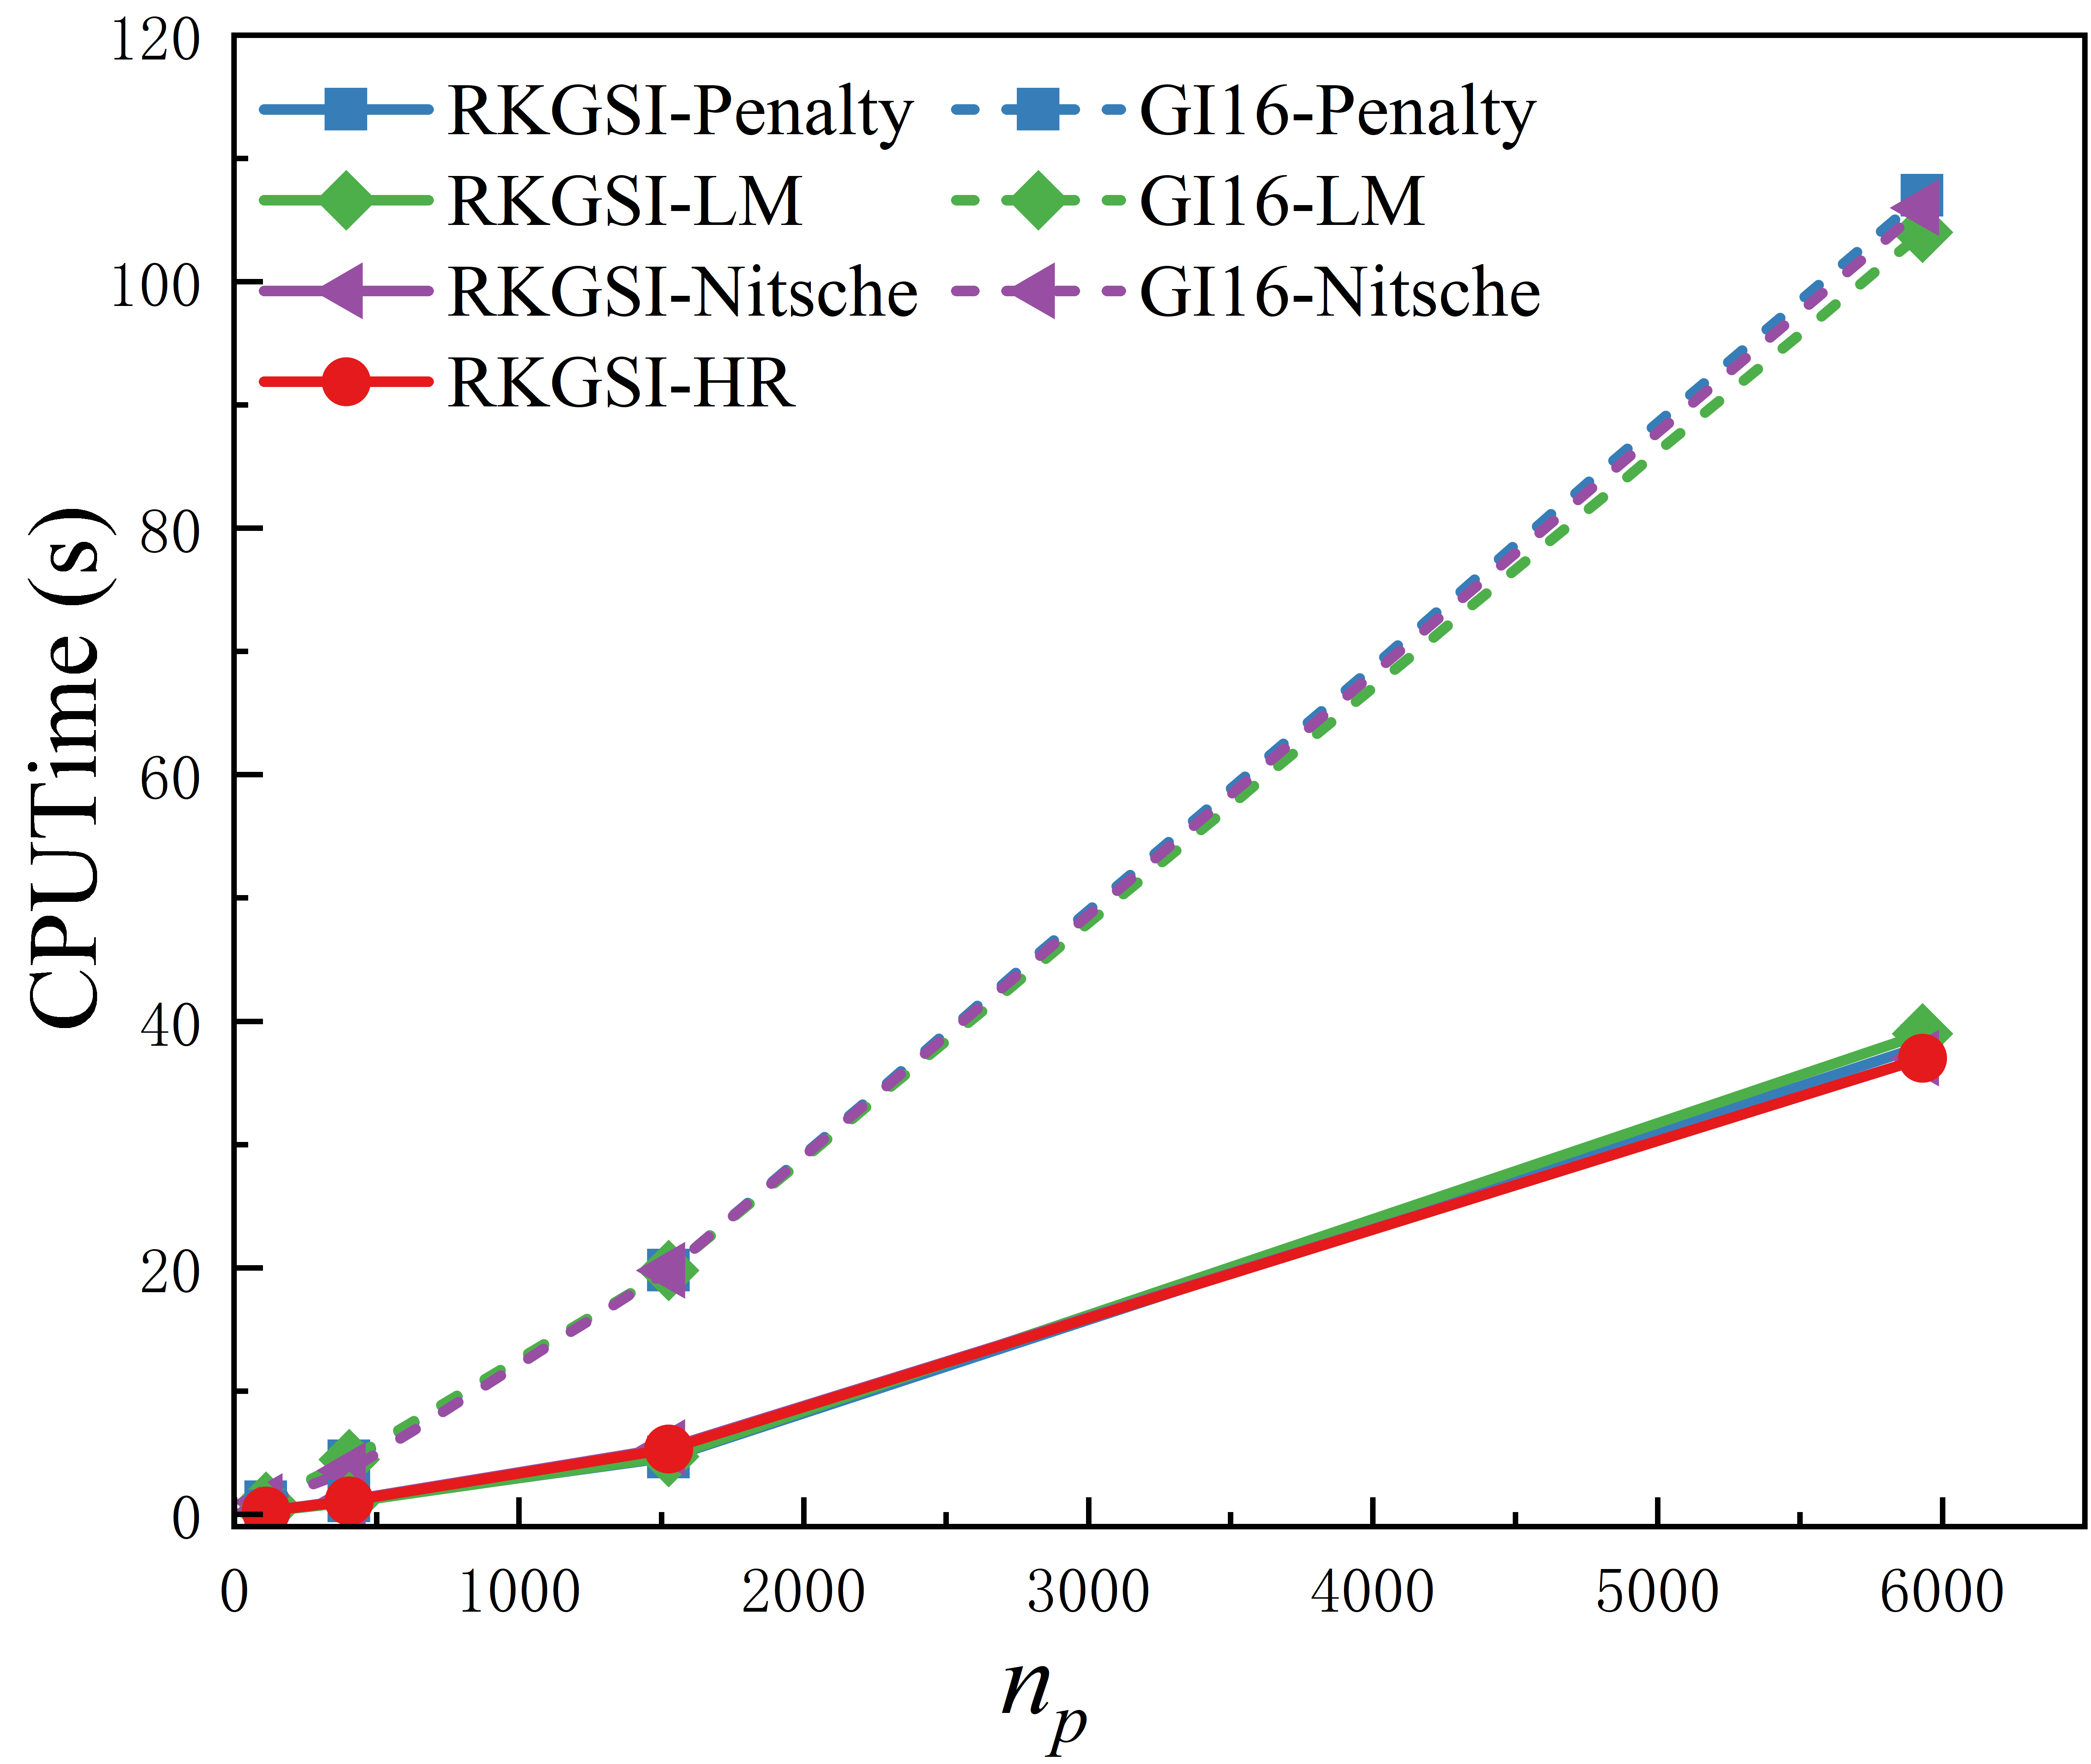
\includegraphics[width=0.49\textwidth]{figure/EHR/hole/cputime.png}
    \phantomcaption\label{Hcputime}
    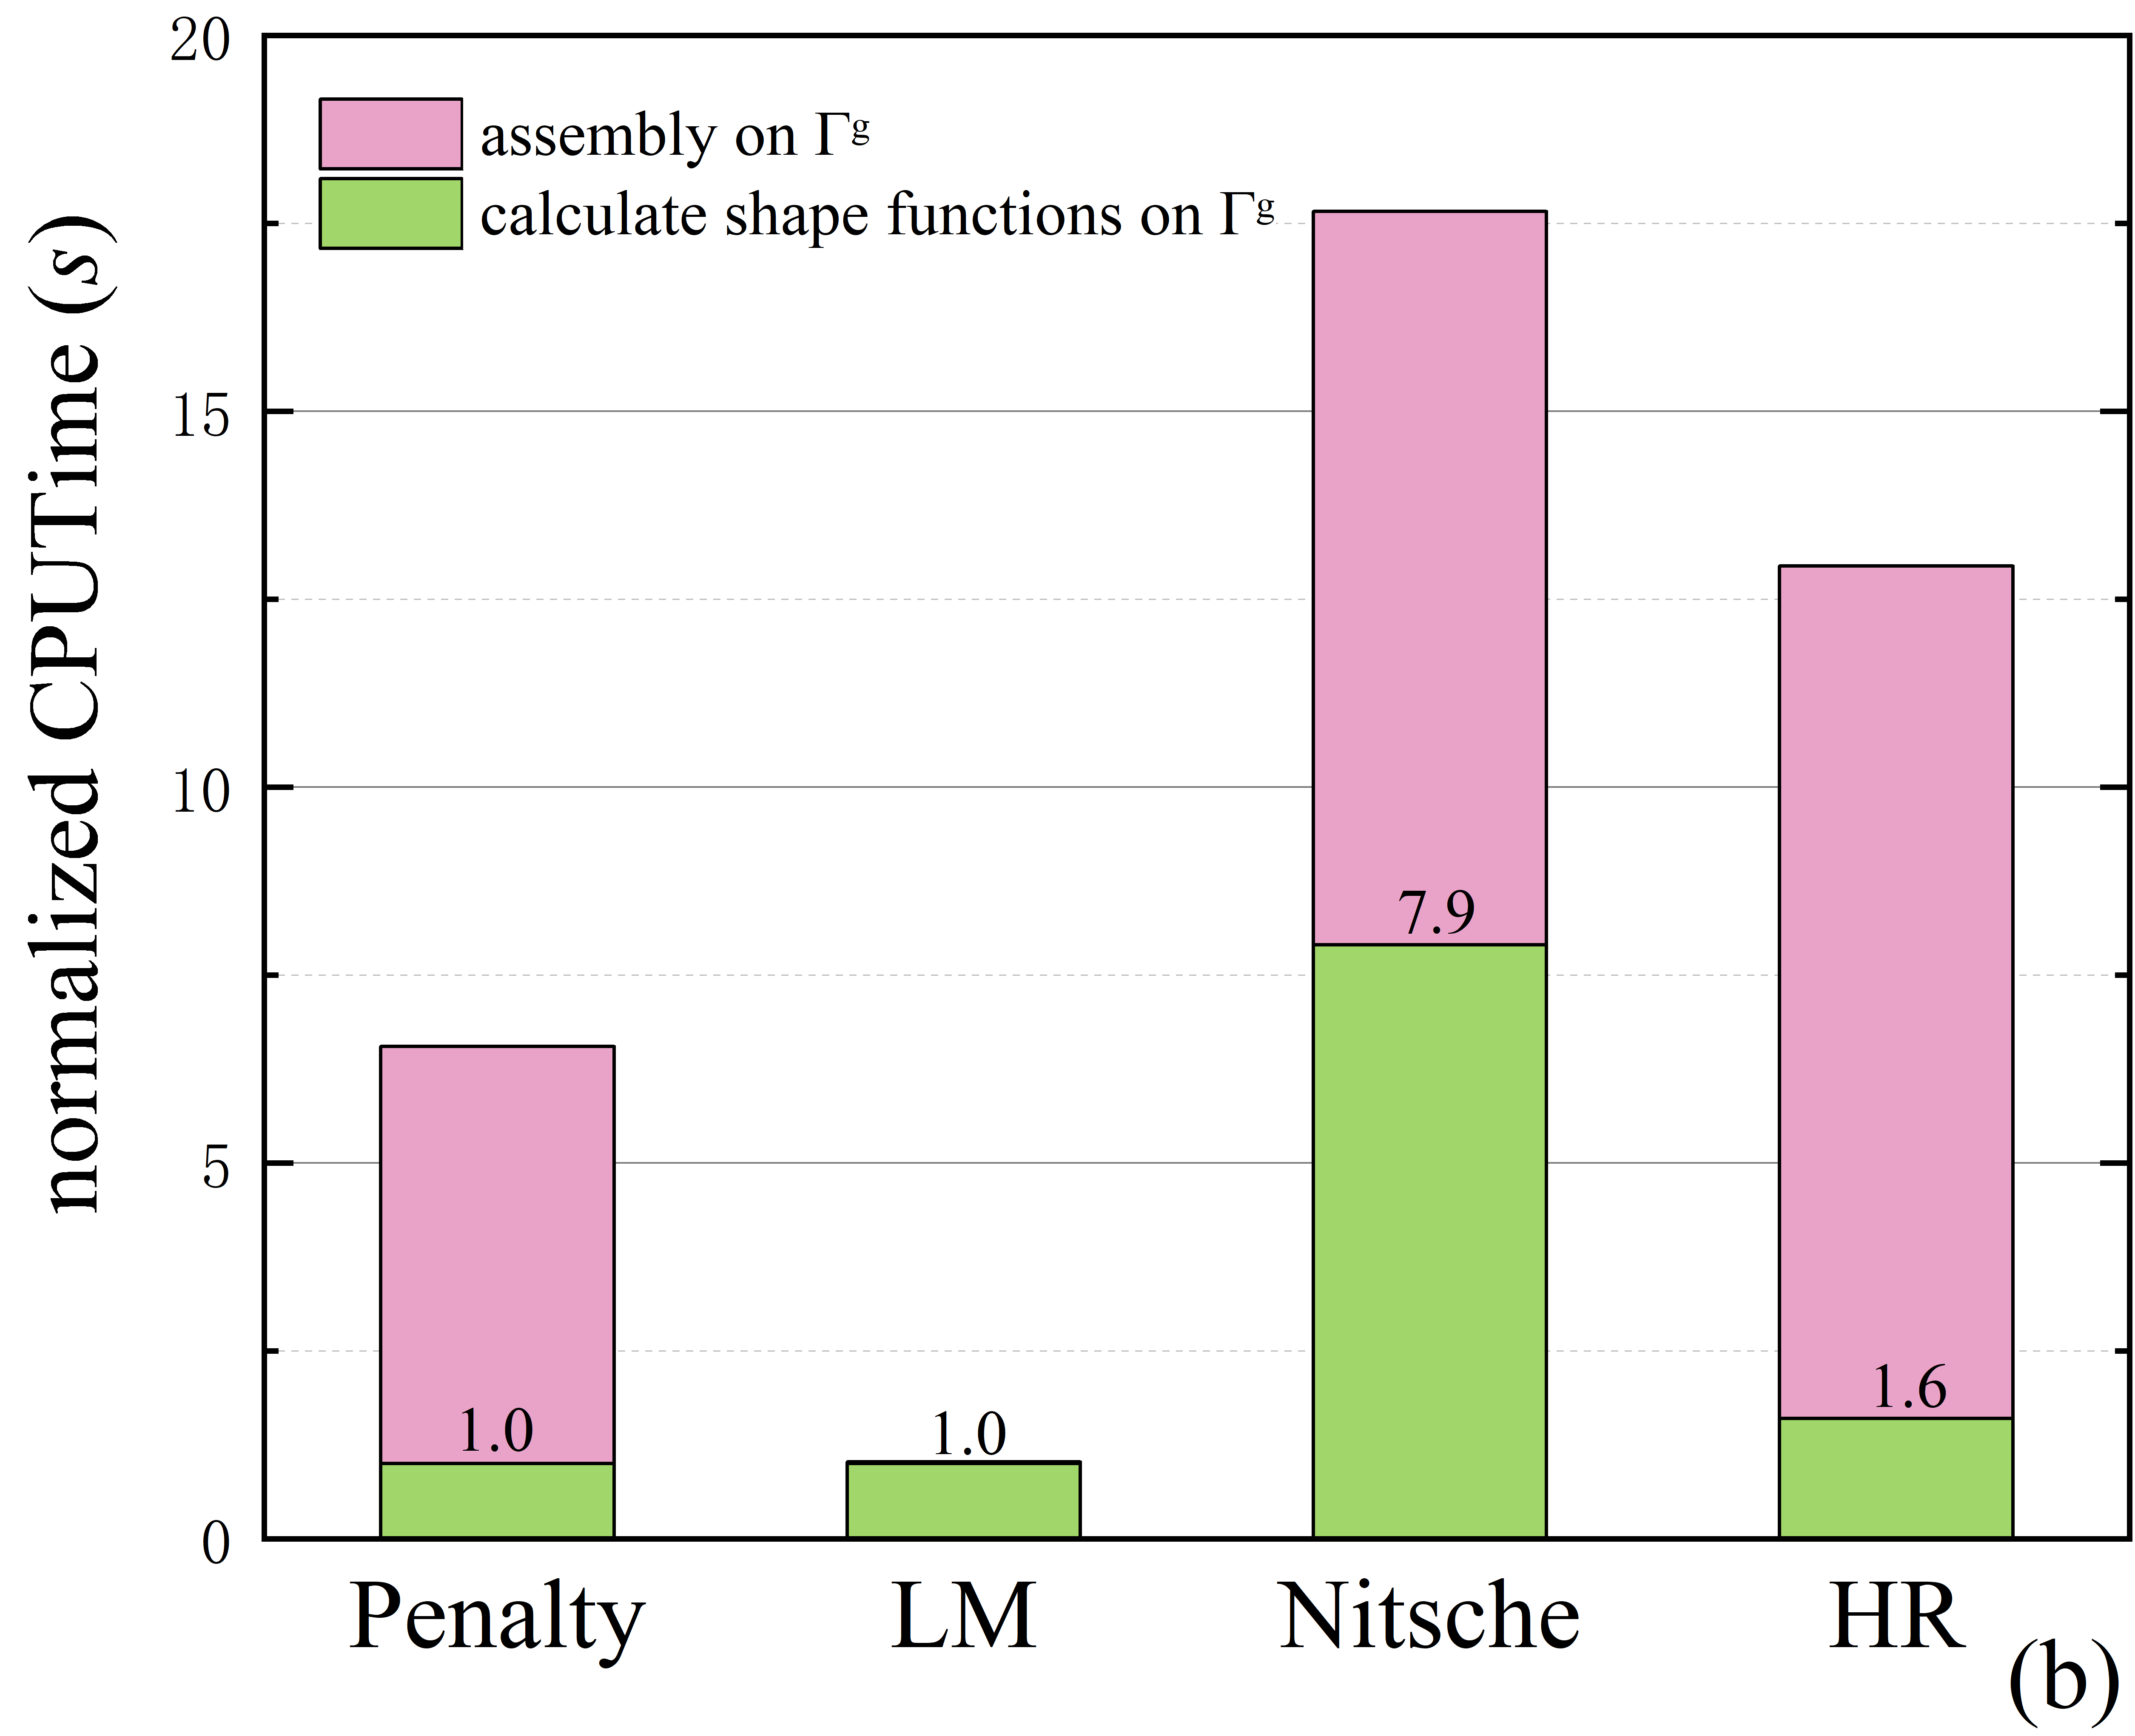
\includegraphics[width=0.49\textwidth]{figure/EHR/hole/efficiency.png}
    \phantomcaption\label{Hefficiency}
\end{subcaptiongroup}
\caption{\centering{带孔无限大平板问题效率对比:\\\subref{Hcputime} 计算时间与节点数的关系;\subref{Hefficiency} 边界条件施加效率分析}}
\end{figure} 
\section{小结}
本章介绍了一种基于Hellinger-Reissner变分原理的变分一致性本质边界条件施加方法,用于求解弹性力学问题。该方法通过采用混合离散近似Hellinger-Reissner变分原理弱形式中的位移和应力,实现了满足积分约束条件的一种本质边界条件施加方法。
具体来说,该方法在离散平衡方程中,采用传统无网格形函数对位移进行离散,而将应力在每个背景积分域上近似为对应阶次的多项式。在Hellinger-Reissner变分原理的框架下,该方法的离散平衡方程具有类似传统Nitsche法的格式,可以视为再生光滑梯度积分法的一种新型Nitsche法。
相较于传统Nitsche法,该方法的修正变分项采用了无网格形函数和再生光滑梯度的混合离散,从而在确保变分一致性的同时避免了复杂且耗时的形函数导数计算,明显提高了计算效率。
与此同时该方法中的稳定项直接源于Hellinger-Reissner变分原理的弱形式,无需额外增加稳定项,并且稳定项中不包含任何人工参数。
这有效消除了传统Nitsche法中人工参数依赖性的问题。
之后进一步通过典型算例的系统验证所提方法基于Hellinger-Reissner变分原理施加本质边界条件的变分一致性、计算精度和计算效率。
结果表明,该方法在保持变分一致性的同时,能够提供较高的计算精度,并且相比传统Nitsche法也有效的提高了计算效率。
\begin{figure}[H]
    \centering
    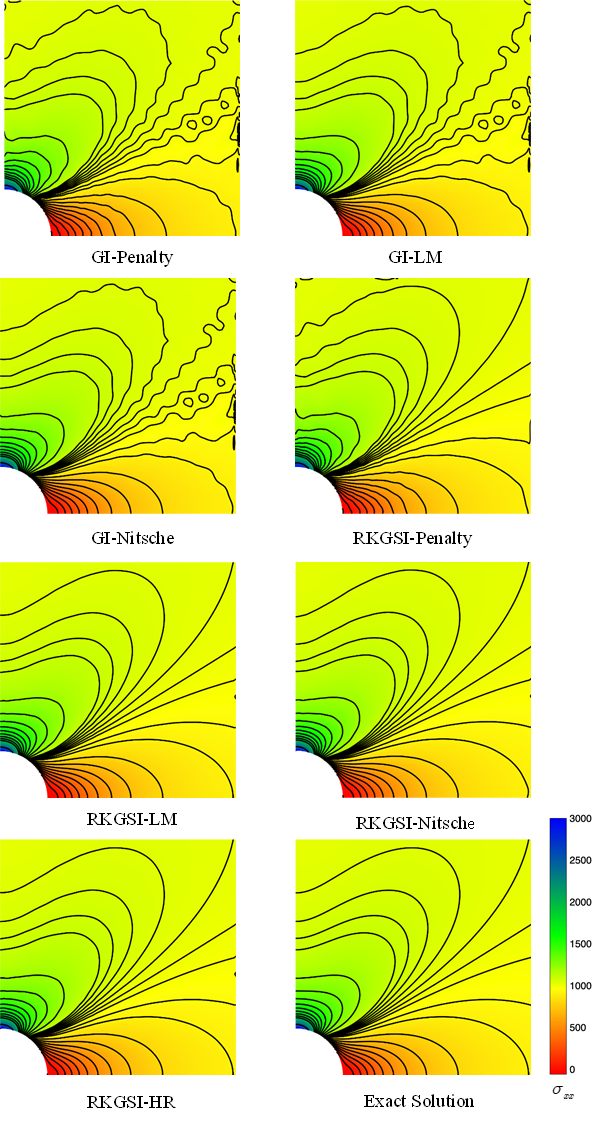
\includegraphics[scale=0.55]{figure/EHR/hole/sigmaxx.png}
\caption{带孔无限大平板问题$\sigma_{xx}$应力云图}\label{sigmaxx}
\end{figure}
